%\documentclass[a4paper,11pt]{book}
\documentclass[a4paper,12pt]{report}
\usepackage[utf8x]{inputenc}
\usepackage{array}
%\documentclass[a4paper,12pt]{article}
% \addtolength{\hoffset}{-1.5cm}
% \addtolength{\textwidth}{3.5cm}
% \addtolength{\voffset}{-1.50cm}
% \addtolength{\textheight}{2.5cm}
% \setlength{\topmargin}{0.25in}
\usepackage[top=1.5in,left=1.5in,right=1in,bottom=1in]{geometry}
\usepackage{amssymb}
\usepackage{amsmath}
%\usepackage{epsfig}
\usepackage[usenames,dvipsnames]{pstricks}
 \usepackage{pst-grad} % For gradients
 \usepackage{pst-plot}
\usepackage{mathptm}
\usepackage{graphics}
\usepackage{graphicx}
\usepackage{amsfonts}
\usepackage{fancyhdr}
%\usepackage{cite}
\usepackage{gensymb}
%\usepackage{fix-cm} %% to change font size
%\usepackage{subfigure}   %%Don't use this package if you are going to use the package {subfig}
\usepackage{rotating}
%\usepackage[usenames,dvipsnames]{color}
\usepackage{shorttoc}
\usepackage{verbatim}
\usepackage{float}
\usepackage{subfig}  %% For placing pictures side by side
\usepackage{fmtcount}
\linespread{1.5}%% To change the distance between lines
%\usepackage[toc]{glossaries}  %% Refer Userguide. Nomenclature is easier to use.
%\usepackage[acronym,toc]{glossaries}
%\makeglossaries

%\usepackage{hyperref}
\usepackage{subfloat}
\usepackage{multirow} %% To combile two or more rows in a table
\usepackage[super]{natbib}
\usepackage[super]{nth} %% For writing 2nd, 3rd, 4th etc by just writing \nth{1}. Requires nth.sty file to be in the working directory.
\newcommand{\tsp}{\textsuperscript} %% For writing kth, nth etc where \nth doesnt work. instead of writing \textsuperscript{th}, just write \tsp{th}
\usepackage{fixltx2e} %% To use the below \textsubscript
\usepackage{xspace}
\usepackage[lined,boxed,linesnumbered]{algorithm2e}
\newcommand{\tsb}{\textsubscript}
\usepackage{nomencl}  %% For Using Symbols and abbreviations. Needs nomencl.sty file to be in the working directory.
\makenomenclature     %% Additional package for nomencl. Search internet for details.
\renewcommand\nomname{SYMBOLS AND ABBREVIATIONS}   %% For changing the Heading from Nomenclature to Symbols and Abbreviations.
%\usepackage{acronym} %% For acronyms
%\usepackage[usenames,dvipsnames]{color}
%\usepackage[round]{natbib}
\usepackage[pagebackref]{hyperref}%\usepackage{hyperref}%% To use hyperlinks to all citations
\hypersetup{
% colorlinks, citecolor=black,
% pagebackref=true,
 linktoc=all,
 hyperindex=true,
 linktocpage=true,
 pdfauthor={Meera Mohan, Narendran Kumaragurunathan},
 pdftitle={Interactive Offline Interface To Debug Simulation Failure, Improved Dual Simulation Approach to Gatesim},
 pdfsubject={VLSI},
 pdfkeywords={Simulation Debug, x86, Gatesim},
 pdfcreator={LaTeX},
 bookmarks=true
}%% Check hyperref manual for details
\usepackage[all]{hypcap} %% To point to the top of the tables and pictures rather than at the bottom


\setlength{\headheight}{15.2pt}
\pagestyle{fancy}
\renewcommand{\sectionmark}[1]{}
%\renewcommand{\chaptermark}[1]{\markboth{\chaptername\ \thechapter.\ #1}{}}
\renewcommand{\chaptermark}[1]{\markboth{\thechapter.\ #1}{}}
%\renewcommand{\footrulewidth}{0.5pt}
\renewcommand{\headrulewidth}{0pt}
\fancyfoot[R]{\textit{Dept. of ECE, NITK Surathkal}}
\fancyfoot[C]{\thepage}

\begin{document}
%\maketitle
%%%%%%%%%%%%%%%%%%%%%%%%%%%%%%%%%%%%%% title page  %%%%%%%%%%%%%%%%%%%%%%%%%%%%%%%%%%%%%%%%%%%%%%%%%%%%%%%%%%%%%%%%%%%%
\begin{titlepage}
\begin{center}
% Title
%\vspace*{3.5cm}
%{\Huge \textbf{MAPPING OF DSP KERNELS ON RECONFIGURABLE PROCESSOR IMPLEMENTED ON FPGA}}\\

{\Large INTERACTIVE OFFLINE INTERFACE TO DEBUG}\\
\vspace{3.5pt}

{\Large SIMULATION FAILURE}\\
\vspace{3.5pt}
{\emph{and}}\\
\vspace{3.5pt}
{\Large IMPROVED DUAL SIMULATION APPROACH}\\
\vspace{3.5pt}
{\Large TO GATESIM}\\
\vspace{5pt}
%%%{\Huge IMPLEMENTED ON FPGA}\\
%%%\vspace{30pt}
%{ \Large Thesis}  \\
Thesis\\
%\vspace{10pt}
{\emph {Submitted in partial fulfillment of the requirements for the degree of}} \\
\vspace{10pt}
{\Large MASTER OF TECHNOLOGY}\\
\vspace{5pt}
%\textit {(by Research)}\\
%\vspace{5pt}
in\\
\vspace{5pt}
{ \Large VLSI DESIGN}\\
\vspace{20pt}
\textit {by} \\
\vspace{10pt}
{\Large MEERA MOHAN}\\ 
{(Reg. No.: 11VL09F)}\\
%Research Scholar\\
%Dept of E \& C, NITK \\
\vspace{1CM}
%\includegraphics*[scale=0.14]{./figures/nitk_logo.ps}\\
\includegraphics*[height=1.5in,width=1.5in]{./figures/Surthkal_logo.eps}\\
\vspace{1cm}
\MakeUppercase{{\large Department of Electronics and Communication Engineering}}\\
\vspace{0.2cm}
\MakeUppercase{{\large National Institute of Technology Karnataka, Surathkal}}\\
\vspace{0.2cm}
\MakeUppercase{{\large Mangalore - 575025}}\\
\vspace{.2cm}
\MakeUppercase{{\large June 2013}}\\
\end{center}
\end{titlepage}
%%%%%%%%%%%%%%%%%%%%%%%%%%%%%%%%%%%%%%%%%%%%%%%%%%%%%%% cover page %%%%%%%%%%%%%%%%%%%%%%%%%%%%%%%%%%%%%%%%
\begin{titlepage}
\begin{center}
% Title
%\vspace*{3.5cm}
{\Large INTERACTIVE OFFLINE INTERFACE TO DEBUG}\\
\vspace{3.5pt}
{\Large SIMULATION FAILURE}\\
\vspace{7pt}
{\emph{and}}\\
\vspace{7pt}
{\Large IMPROVED DUAL SIMULATION APPROACH}\\
\vspace{3.5pt}
{\Large TO GATESIM}\\
%%%{\Huge IMPLEMENTED ON FPGA}\\
%%%\vspace{30pt}
%{ \Large Thesis}  \\

\vspace{15pt}
\textit {by} \\
\vspace{10pt}
{\Large {Meera Mohan}}\\ 
{(Reg. No.: 11VL09F)}\\
%Research Scholar\\
%Dept of E \& C, NITK \\
\vspace{15pt}
{\em Under the Guidance of} \\
\vspace{10pt}
\hspace{-0.35in}{\Large {Dr. M. S. Bhat \hspace{1.5in} Mr. Narendran. K }} \\
\hspace{-0.05in} Professor \hspace{2in} SMTS Design Engineer\\
\hspace{-0.45in}Dept of E \& C, NITK \hspace{1.65in} AMD India Pvt. Ltd\\

%\vspace{10pt}
%{\Large {Dr. M. S. Bhat \hspace{1in} Mr. Narendran. K}} \\
%\hspace{-0.05in} Professor \hspace{2in} SMTS Design Engineer\\
%\hspace{-0.05in}Dept of E \& C, NITK \hspace{1.5in} AMD India Pvt. Ltd\\
\vspace{-0.05in}
\begin{table}[h!]
   \hspace{.3in}  \begin{tabular}{ccc}	
	 			
        \hspace{.5cm}  \begin{minipage}{.5\textwidth}
      
\includegraphics[width=0.85in, height=0.85in]{./figures/Surthkal_logo.eps}
    \end{minipage}
    &
    \begin{minipage}{.5\textwidth}
		
\includegraphics[width=1.2in, height=0.6in]{./figures/amd_logo.eps}
     \end{minipage}
      \end{tabular}
%\caption*{logo}
 \end{table}

%\vspace{10pt}
%\hspace{-.5in}{\Large {Dr. M. S. Bhat \hspace{2in} Mr. Narendran. K}} \\
%\hspace{-1.4in}Professor \hspace{2.50in} SMTS Design Engineer\\
%
%\hspace{-0.45in}Dept of E \& C, NITK \hspace{1.65in} AMD India Pvt. Ltd\\
\vspace{-0.25in}
%\begin{figure*}[htp]
%\hspace{0.6in} \subfigure{
\includegraphics[height=0.85in,width=0.85in]{./figures/Surthkal_logo.eps}}\hspace{2.1in}
%   \subfigure{
\includegraphics[height=0.6in,width=1.2in]{./figures/amd_logo.eps}}
%\end{figure*}

\
 {Thesis}  \\
{\emph {Submitted in partial fulfillment of the requirements for the degree of}} \\
\vspace{10pt}
{\Large {MASTER OF TECHNOLOGY}}\\
\vspace{5pt}
%\textit {(by Research)}\\
%\vspace{5pt}
in\\
\vspace{5pt}
{ \Large {VLSI DESIGN}}\\
\vspace{.5cm}
{\Large Department of Electronics and Communication Engineering }\\
\vspace{0.2cm}
{\Large National Institute of Technology Karnataka, Surathkal}\\
\vspace{0.2cm}
{\Large Mangalore - 575025}\\
\vspace{0.5cm}
{\large June 2013}\\
\end{center}
\end{titlepage}

%%%%%%%%%%%%%%%%%%%%%%%%%%%%%%%%%%%%%%%% DECLARATION %%%%%%%%%%%%%%%%%%%%%%%%%%%%%%%%%%%%%%%%%
\newpage
\thispagestyle{empty}
\section*{\centering DECLARATION}
\begin{center}
 \emph{by the M.Tech student}
\end{center}
I hereby \emph{declare} that the Report of the P.G. Project Work entitled 
{\bf Interactive Offline Interface To Debug Simulation Failure} and {\bf  Dual Simulation Approach To Gatesim}
which is being submitted to {\bf National Institute of Technology Karnataka, Surathkal}, 
in partial fulfillment for 
the requirements of the award of degree of {\bf Master of Technology} 
in {\bf VLSI Design} in the department of {\bf Electronics and Communication Engineering}, 
is a \emph{bonafide report of the work carried out by me}. The material contained 
in this report has not been submitted at any other University or Institution 
for the award of any degree.

\vspace{1.2in}
\begin{flushright}
 11VL09F, Meera Mohan, .........................\\
 (Register Number, Name and Signature of the student)\\
\vspace{1cm}
Department of Electronics and Communication Engineering
\end{flushright}

\vspace{0.2in}
\begin{flushleft}
 Place : NITK, Surathkal\\
 Date  :
\end{flushleft}

%%%%%%%%%%%%%%%%%%%%%%%%%%%%%%%%%%%%%%% CERTIFICATE %%%%%%%%%%%%%%%%%%%%%%%%%%%%%%%%%%%%%%%%%
\newpage
\thispagestyle{empty}
\section*{\centering CERTIFICATE}
This is to \emph{certify} that the Post Graduation Project Work Report entitled 
{\bf Interactive Offline Interface To Debug Simulation Failure} and {\bf Dual Simulation Approach To Gatesim} 
submitted by {\bf Meera Mohan} (Register number: 11VL09F) as the 
record of the work carried out by him/her, is \emph{accepted as the  
P.G Project Work Report submitted} in partial fulfillment for 
the requirements of the award of degree of {\bf Master of Technology} 
in {\bf VLSI Design} in the department of {\bf Electronics and Communication} 
at {\bf National Institute of Technology Karnataka, Surathkal} during the 
academic year 2012-2013.

\vspace{1.4in}

 \begin{tabular}{lll}
 \hspace{-1cm}\bf{Mr. Narendran Kumaragurunathan}	&\hspace{.7cm}\bf{Prof. M. S. Bhat}	 &\hspace{.7cm}\bf{Prof. Muralidhar Kulkarni}	\\
 \hspace{-1cm}\bf{Project Guide} &\hspace{.7cm}\bf{Project Guide}		&\hspace{.7cm}\bf{Chairman DPGC}
\end{tabular}
 %\begin{minipage}[b]{.5\linewidth}
%  \begin{flushleft}
%  \bf{Ramesh Kini M.}\\
%  \bf{Project Guide}
%  \end{flushleft}
%\end{minipage}

%\hspace{.5cm}

%\begin{minipage}[b]{.5\linewidth}
%   \begin{flushright}
%   \bf{Dr. Muralidhar Kulkarni}\\
%   \bf{Chairman DPGC}
%   \end{flushright}
%\end{minipage}









%%%%%%%%%%%%%%%%%%%%%%%%%%%%%%%%%%%%%%% ACKNOWLEDGMENTS %%%%%%%%%%%%%%%%%%%%%%%%%%%%%%%%%%%%%%%%%
\newpage
\pagenumbering{roman}
\pagestyle{plain}
%%%\section*{\centering ACKNOWLEDGMENTS}
The success of a project requires help and contribution from numerous individuals and 
the organization. Writing the report of this project work gives me an opportunity to 
express my gratitude to everyone who has helped in shaping up the final outcome of my 
project work.
 \paragraph{} I express my heartfelt gratitude to my project guide {\bf Dr. M. S. Bhat.} for 
giving me an opportunity to do my major project work under his guidance. His constant 
support and encouragement has made me realize that it is the process of learning which 
weighs more than the end result.

\paragraph{}I am highly indebted to my external guide, {\bf Mr. Narendran Kumaragurunathan}, Senior Member Technical Staff, AMD India Pvt Ltd, for
his guidance, constant supervision and for motivating me to complete my work.
He helped me throughout by giving new ideas, providing necessary information and
pushing me forward to finish the project work. 

\paragraph{} Many thanks to {\bf Dr. John D'Souza}, M.Tech Project Co-coordinator, Department of 
Electronics and Communication, for his valuable suggestions and help.
\paragraph{} I would like to thank all the team members of SoC Verification Team at AMD India Pvt Ltd, Bangalore for their support and help through out the course of my work there.
\paragraph{} My deep gratitude to my family and friends who have stood by me at all times, motivating 
me and bearing my mood swings. Many thanks to all who have helped me, directly or indirectly, in 
the successful completion of my project work
%has helped me push myself through rough times.

\addcontentsline{toc}{section}{ACKNOWLEDGEMENTS}
%%%%%%%%%%%%%%%%%%%%%%%%%%%%%%%%%%%%%%%%%%%%%%%%%%%%%% ABSTRACT %%%%%%%%%%%%%%%%%%%%%%%%%%%%%%%%%%%%%%%%%
\newpage
\pagestyle{plain}
\section*{\centering ABSTRACT}
\newcommand{\RNum}[1]{\uppercase\expandafter{\romannumeral #1\relax}}


\centerline{\emph{\bf PART \RNum{1}- Interactive Offline Interface To Debug Simulation Failure }}
\vspace{5pt}
Processor execution log contains in depth details pertaining to processor execution.  These files hold instruction by instruction execution details and status information.  In the event of a simulation failure, debugging requires tracing through the execution logs for failure diagnosis.  Due to the significant information contained in these log files, it becomes overwhelming to comprehend it quickly because relevant information is spread across in different files and manual tracing is a tedious job.


This project aims to implement a graphic user interface for faster and effortless tracing through the log files.  The interface gathers all the relevant data related to execution flow and represents correlated information as appropriate to user.  The graphic interactive navigation windows tries to reduce the user's time spends on tracing cause of failure.   



\paragraph{Keywords:}
 \emph{Debug Interface, Execution Log Files, SoC  Verification.}


 \paragraph{}

\centerline{\emph{\bf PART \RNum{2}- Dual Simulation Approach To Gatesim}}
\vspace{5pt}
Gatesim or gate level simulation verification focuses on verifying the post layout netlist of a module. Gatesim verification is an important milestone and confidence builder for verification. Multiple methodologies are in existence in the industry for this purpose. In AMD, Gatesim verification uses co-simulation methodology for the purpose, where full chip behavioral RTL and gate netlist is simulated simultaneously in one simulation. Verification is done by driving corresponding RTL stimulus onto netlist and by comparing response every cycle. 
The objective of this project is to improve the simulation, turn-around times and resource requirements involved in Gatesim verification without compromising on verification. The thesis proposes a new dual simulation approach to Gatesim where RTL and gate level simulation happens separately and test vectors for netlist simulation is read from database generated during RTL simulation. The approach thrives to overcome performance issues with current co-simulation methodology.

\paragraph{Keywords:}
 \emph{Gatesim,  GLS,  Co-simulation Methodology,  Functional Verification, Netlist Simulation.}



\addcontentsline{toc}{section}{ABSTRACT} 

%%%%%%%%%%%%%%%%%%%%%%%%%%%%%%%%%%%%%% TABLE OF CONTENTS %%%%%%%%%%%%%%%%%%%%%%%%%%%%%%%%%%%%%%%%%%%%%%%
\newpage
%\pagestyle{plain}
\tableofcontents 
\addcontentsline{toc}{section}{CONTENTS}

%%%%%%%%%%%%%%%%%%%%%%%%%%%%%%%%%%%%%% LIST OF FIGURES %%%%%%%%%%%%%%%%%%%%%%%%%%%%%%%%%%%%%%%%%%%%%%%%%
\newpage
%\pagestyle{plain}
\listoffigures
\addcontentsline{toc}{section}{LIST OF FIGURES}

%%%%%%%%%%%%%%%%%%%%%%%%%%%%%%%%%%%%%% LIST OF TABLES %%%%%%%%%%%%%%%%%%%%%%%%%%%%%%%%%%%%%%%%%%%%%%%%%
\newpage
\listoftables
%\pagestyle{plain}
\addcontentsline{toc}{section}{LIST OF TABLES}

%%%%%%%%%%%%%%%%%%%%%%%%%%%%%%%%%%%%%% LIST OF TABLES %%%%%%%%%%%%%%%%%%%%%%%%%%%%%%%%%%%%%%%%%%%%%%%%%
\newpage
\addcontentsline{toc}{section}{LIST OF ALGORITHMS}
\listofalgorithms

%%%%%%%%%%%%%%%%%%%%%%%%%%%%%%%%%%%%%% Symbols and Abbreviations %%%%%%%%%%%%%%%%%%%%%%%%%%%%%%%%%%%%%%%%%%%%%%%%%
\newpage
\printnomenclature
\addcontentsline{toc}{section}{SYMBOLS AND ABBREVIATIONS}





%%%%%%%%%%%%%%%%%%%%%%%%%%%%%%%%%%%%%%%%% PART I : GUI %%%%%%%%%%%%%%%%%%%%%%%%%%%%%%%%%%%%%%%%%%%%%%%%%%%%%%%%%%%%%%
\newpage
\pagestyle{fancy}
\pagenumbering{arabic}
\part{}




%%%%%%%%%%%%%%%%%%%%%%%%%%%%%%%%%%%%% INTRODUCTION %%%%%%%%%%%%%%%%%%%%%%%%%%%%%%%%%%%%%%%%%%%%%%%%%%%
\newpage
\chapter{INTRODUCTION}
%\section{Background}
%\section{Purpose/Motivation}
%\section{Approach}
%\section{Main Contributions}
%\section{Organization of thesis}

With rapid growth of deep sub micron technology, there has been an aggressive shrinking in physical dimension of silicon structures, that can be realized on silicon. This advancement has enabled the transition of multi-million gate designs from large printed circuit boards to SoC (System on Chip) \nomenclature{SoC}{System on Chip}. SoC design has the advantages of smaller size, low power consumption, reliability, performance improvement and low cost per gate. Another major high point of SoC from design point of view is that SoC allows use of predesigned blocks called semiconductor intellectual property (IP) \nomenclature{IP}{intellectual Property}. These hardware IP blocks can be mix-and-matched, thereby providing design reuse in SoC and thereby reducing time-to-market. 


 Over the past few years, major challenges faced by semiconductor industry is to develop more complex SoCs with greater functionality and diversity with reduction in time-to-market. One of the main challenge among this is verification. Integration between various components, combined complexity of multiple sub-systems, software-hardware co-verification, conflicts in accessing shared resource, arbitration problems and dead-locks, priority conflicts in exception handling etc makes SoC verification very hard. It is said that verification consumes more than 60 percent of design effort. This can be easily explained as there is no single design tool that can completely verify a SoC on it's own. Instead a complex sequence of tools and techniques, including simulation, directed and random verification and formal verification are used to verify a SoC. Achieving cent percent functional verification coverage is next to impossible due to time-to-market constraints.


\section{VERIFICATION METHODS}
Two widely adopted verification methodologies are stimulus based dynamic verification methodology and static formal verification methodology. In stimulus based verification the verification engineer develops a set of tests, based on design specifications. Design correctness is then established through simulations. Formal verification is a mathematical proof method of ensuring that a design's implementation matches its specification. The most prominent distinction between stimulus-based verification and formal verification is that the former requires input vectors and the latter does not. In stimulus based verification the idea is to first generate input vectors and then derive the reference output where as in formal verification process it is the reverse approach.

In formal verification the behavior of design is captured as a set of mathematical equations called properties and then the formal verification tool proves or disproves each property appropriately. In formal verification, user need not generate stimulus but specification of invalid stimulus would be necessary.  At SoC level the designs are huge, typically beyond the capacities of automatic formal tools. Formal methodology tools have large memory and long run time requirements. When memory capacity is exceeded, tools often shed little light on what went wrong, or give little guidance to fix the problem. As a result, formal verification software, is best suited only to circuits of moderate size, such as blocks or modules. 

\section{SoC VERIFICATION}
Most SoCs are built around one or more processing cores (multi processor) and verification is done using stimulus based verification methodology where the design model is simulated using random or handwritten test programs. Reference models are simulated in parallel with the design and results are compared.  Comparison between the design architecture state and the reference model states are done after each instruction retire. Difference detected in states is considered as ``{\it mismatches}''. Memory contents are compared at the end of simulation and any discrepancies are reported as ``{\it memory mismatches}''.  The simulator writes entries for each event it processes into processor execution log file.

On event of a simulation mismatch, the processor execution log entries are helpful in understanding and tracing the cause associated with the failure. Logs contain in-depth details pertaining to processor execution. 

\section{PROPOSED ENHANCEMENT TO AID PROCESSOR EXECUTION DEBUG}
Tracing a typical failure is a manual process and is time consuming since relevant informations are buried under a wealth of information, and related informations are spread across in different files. This greatly challenges an engineer's ability to debug and converge on the cause. If there exists a representation which correlates different information and presents them as required by the user, it would aid debug significantly. The proposed interactive interface provides graphical data representations and navigation, helping in faster tracing through processor execution. Such represented information is correlated, filtered and sorted making debugging a lot more intuitive than existing manual method.


Such an envisioned graphical user interface is proposed to aid processor execution debug by representation of data to user. This interface would have properties of a software debugger, and it would work offline. This project work concentrates on implementing such an enhancement.

 


\section{ORGANIZATION OF THE THESIS}
The organization of this project report is as follows:\\
\noindent 
{\bf Chapter}~\ref{chap:amd64}-{\it AMD64 Architecture Overview} gives brief introduction to AMD64 architecture.\\
{\bf Chapter}~\ref{chap:verification.tex}-{\it Verification Shortfalls} discusses existing verification methodologies and their shortfalls.\\
{\bf Chapter}~\ref{chap:enhancement.tex}-{\it Proposed Enhancement} discusses desired features of proposed enhancement.\\
{\bf Chapter}~\ref{chap:GUI_impl.tex}-{\it Implementation of Proposed Enhancement} gives implementation details of proposed enhancement.\\
{\bf Chapter}~\ref{chap:GUI_results.tex}-{\it Implementation Results} a final look at the implemented enhancement.\\
%{\bf Chapter}~\ref{chap:conclusion} discusses the various 
%conclusion drawn from the results and the scope for future work.



%%%%%%%%%%%%%%%%%%%%%%%%%%%%%%%%%%%%%% AMD64 %%%%%%%%%%%%%%%%%%%%%%%%%%%%%%%%%%%%%%%%%%%%%%%
\newpage
\chapter{AMD64 ARCHITECTURE OVERVIEW}
\label{chap:amd64}
Typically a SoC brings together functionality that used to be distributed across chips or maybe even devices. Various functional modules of the system are integrated into a single chip set. Naturally SoCs are very complex designs which includes programming elements, hardware elements, software elements, bus architecture, clock and power distribution, test structures etc. 

The heart of any SoC design is a core which is nothing but some sort of processor, and practically all SoC is likely to have at least one processor. In AMD, most processors are based on AMD64 architecture. Majority of the verification scenarios are developed in reference to the behavior of core and hence makes it an important design of interest.

\section {AMD64 ARCHITECTURE}
The AMD64, originally called x86-64, architecture is a 64-bit, backward compatible extension of industry-standard x86 architecture (legacy)~\citep{SS:AMD64-V1}. It adds 64-bit addressing and expands register resources to support higher performance for recompiled 64-bit programs, while supporting legacy 16-bit and 32-bit applications and operating systems without modification or recompilation. The need for a 64 bit x86 architecture is driven by applications that address large amounts of virtual and physical memory, such as high-performance servers, database management systems, and CAD tools. These applications benefit from both 64-bit addresses and an increased number of registers.



\section {FEATURES OF AMD64}
\addtocontents{toc}{\protect\setcounter{tocdepth}{1}}
The main features of AMD64 architecture are its extended 64-bit registers and new 64-bit mode of operation.  
\subsection{REGISTERS}

One of the main features of AMD64 architecture is the 64-bit register extension. The small number of registers available in the legacy x86 architecture limits performance in computation-intensive applications. Increasing the number of registers provides a performance boost to many such applications. In addition to the 8 legacy x86 General-Purpose Registers (GPRs), AMD64 introduce additional 8 GPRs. All 16 GPRs are 64-bit long and an instruction prefix (REX) accesses the extended registers. The architecture also introduces 8 new 128-bit media registers.
%\figurename{} 
\begin{figure}[h!]
\centering
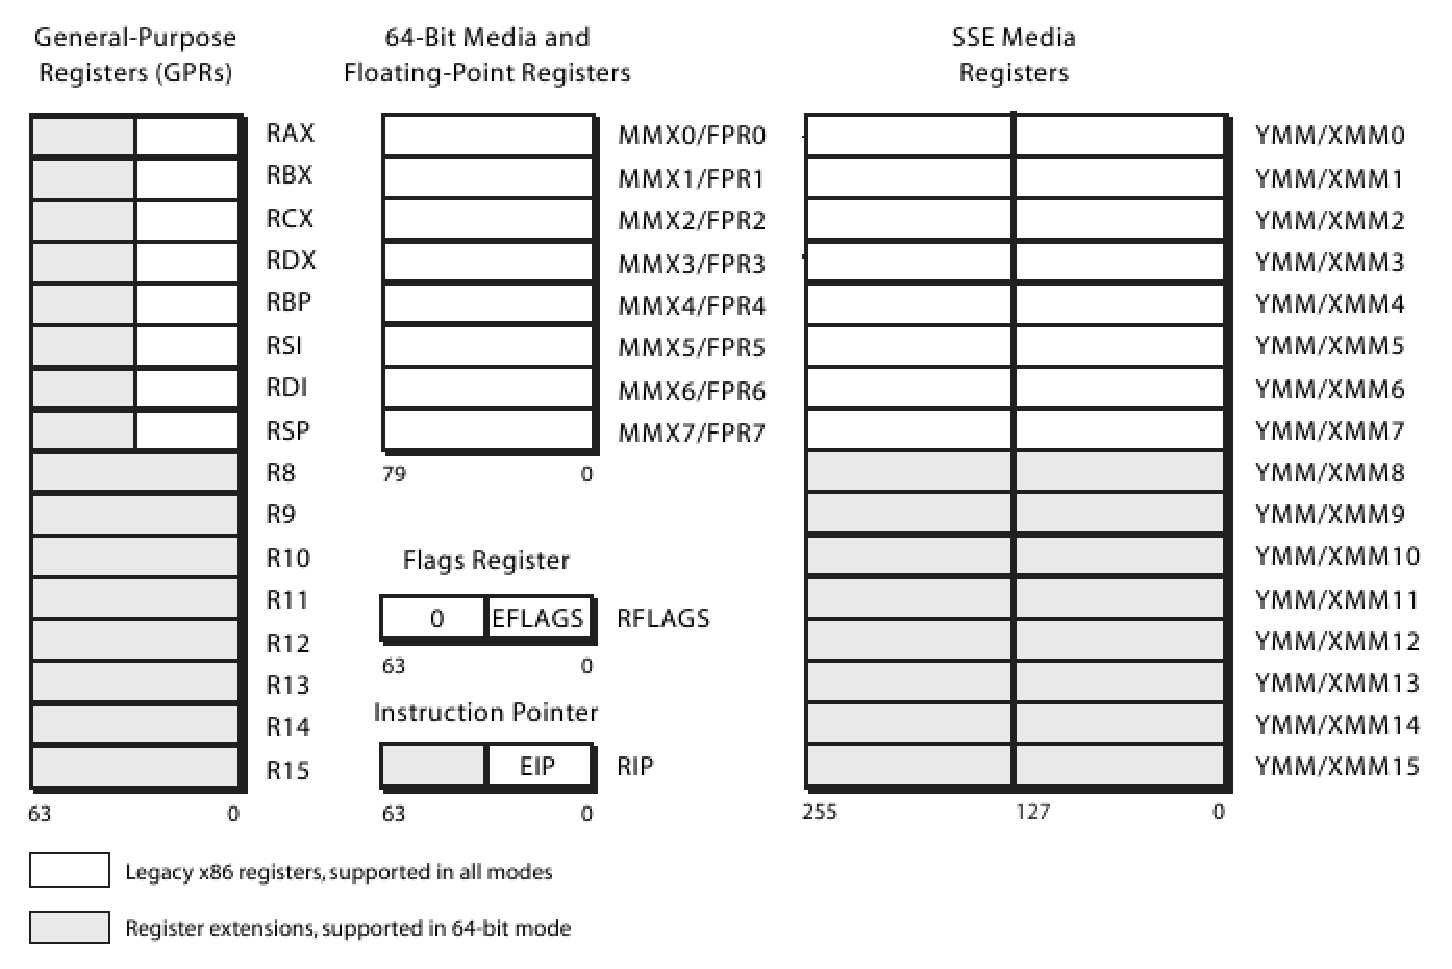
\includegraphics[scale=0.65]{./figures/registers.eps}
\caption{AMD64 Registers}
\label{fig:registers.eps}
\end{figure}


~\figurename{~\ref{fig:registers.eps}} shows the AMD64 application-programming register set. They include the general-purpose registers (GPRs), segment registers, flags register (64-bits), instruction-pointer register (64-bits) and the media registers. 

\subsection{MODES OF OPERATION}
In addition to the x86 legacy mode, another major feature of AMD64 for is its long mode. This is the mode where a 64-bit application (or operating system) can access 64-bit instructions and registers.%~\figurename{~\ref{fig:modes.eps}} shows the features of each mode of operation in AMD64 architecture. 
The different modes of operations in AMD64 architecture are detailed below:
%\begin{tabular}
%\figurename{} 
%\begin{figure}[h!]

%\centering
%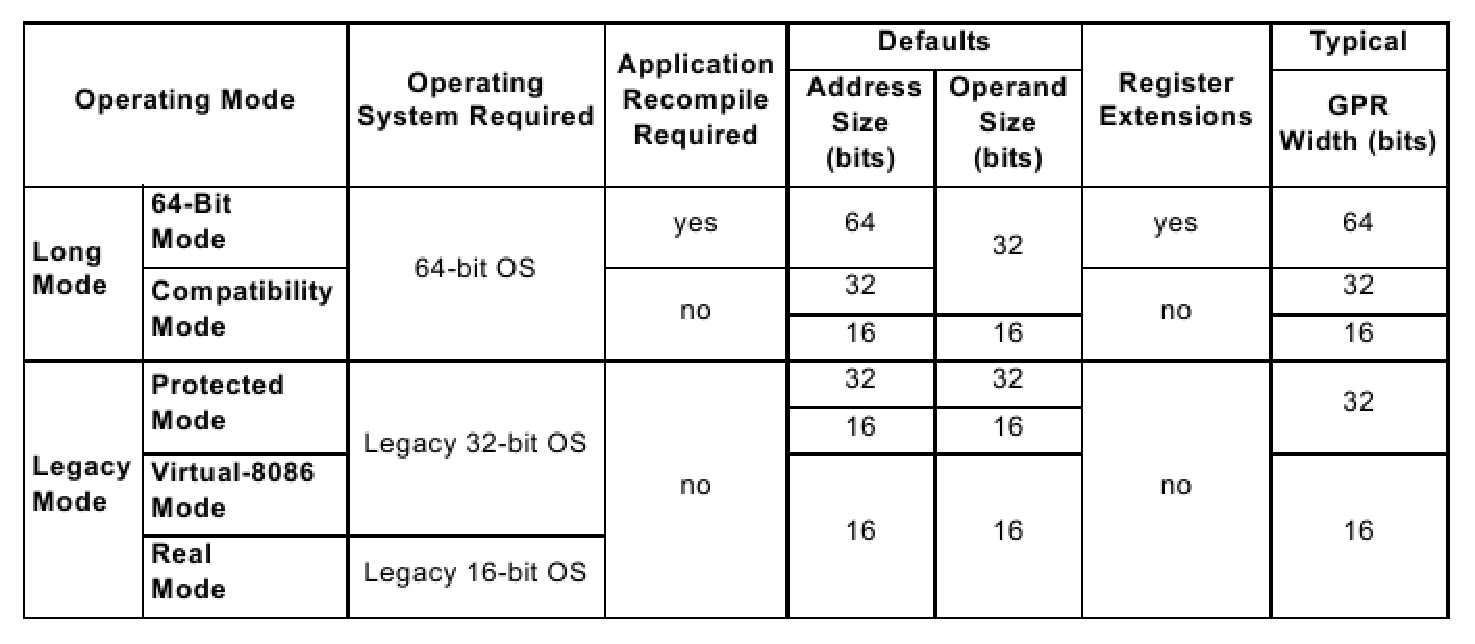
\includegraphics[width=6in]{./figures/modes.eps}
%\caption{AMD64 Modes of Operation}
%\label{fig:modes.eps}
%\end{figure}
%\end{tabular}



\emph {\bf Long Mode}: Long mode is an extension of legacy protected mode. It consists of two sub modes: 64-bit mode and compatibility mode. 64-bit mode supports all of the new features and register extensions of the AMD64 architecture. Compatibility supports binary compatibility with existing 16-bit and 32-bit applications. Long mode does not support legacy real mode or legacy virtual-8086 mode, and it does not support hardware task switching.
\begin{itemize}

\item 64-bit mode: 64-bit mode supports the full range of 64-bit virtual-addressing and register-extension features. This mode is enabled by the operating system on an individual code segment basis. As 64-bit mode supports a 64-bit virtual-address space, it requires a 64-bit operating system and tool chain.


\item Compatibility Mode: Compatibility mode allows 64-bit operating systems to run existing 16-bit and 32-bit x86 applications. These legacy applications run in compatibility mode without recompilation. This mode is also enabled by operating system on an individual code segment bases as in 64 bit mode. However unlike 64-bit mode, x86 segmentation function similar to legacy x86 architecture using 16-bit or 32-bit protected mode semantics.

\end{itemize}



\emph {\bf Legacy Mode}: Legacy mode has compatibility existing 16-bit and 32-bit operating systems in addition to compatibility with existing 16-bit and 32-bit application. Legacy mode has the following three submodes : 

\begin{itemize}

\item Protected Mode: Legacy protected mode supports 16-bit and 32-bit programs with memory segmentation, optional paging, and privilege-checking. Programs in this mode can access up to 4GB of memory space.


\item Virtual-8086 Mode: Virtual-8086 mode supports 16-bit real-mode programs running as tasks under protected mode. It uses a simple form of memory segmentation, optional paging and limited protection-checking. Programs in virtual-8086 mode can access up to 1MB of memory space.


\item Real Mode: Real mode supports 16-bit programs using register-based memory segmentation. It does not support paging or protection-checking. Programs running in real mode can access up to 1MB of memory space.
\end{itemize}

\section{MEMORY ORGANIZATION}
\addtocontents{toc}{\protect\setcounter{tocdepth}{1}}

The AMD64 architecture organizes memory into virtual memory and physical memory~\citep{SS:AMD64-V2}. Virtual memory and physical-memory spaces are usually different in size with virtual address space being much larger than physical-address memory.  System software relocates applications and data between physical memory and the system hard disk to make it appear that much more memory is available than what really exist and then uses the hardware memory-management mechanisms to map the larger virtual-address space into the smaller physical-address space.

\subsection {VIRTUAL MEMORY}
Virtual memory consists of the entire address space available. It is a large linear address space that is translated to a smaller physical address space. Programs uses virtual address space to access locations within the virtual memory space. System software is responsible for managing the relocation of applications and data in virtual memory space using segment-memory management. System software is also responsible for mapping virtual memory to physical memory through the use of page translation.

The architecture supports different virtual-memory sizes using the following modes:
\begin{itemize}

\item[-] Protected Mode: Supports 4 gigabytes of virtual-address space using 32-bit virtual  addresses.

\item[-] Long Mode: Supports 16 exabytes of virtual-address space using 64-bit virtual addresses.
\end{itemize}

\subsection {PHYSICAL MEMORY}
Physical addresses are used to directly access main memory. This is the installed memory in a particular system that can be physically accessed by the bus interfaces. The larger virtual address space is translated to smaller physical address space through two translation stages called segmentation and paging. The architecture supports different physical-memory sizes using the following modes:
\begin{itemize}

\item[-] Real Mode- Supports 1 Megabyte of physical-address space using 20-bit physical addresses.
\item[-] Legacy Protected Mode- Supports several different address-space sizes, depending on the translation. supports 4 gigabytes of physical address space using 32-bit physical addresses and when the physical-address size extensions are enabled, the page-translation mechanism can be extended to support 52-bit physical addresses.
\item[-] Long Mode- Supports up to 4 petabytes of physical-address space using 52-bit physical addresses. Long mode requires the use of page-translation and the physical-address size extensions (PAE).
\end{itemize}

\section{MEMORY MANAGEMENT}

\addtocontents{toc}{\protect\setcounter{tocdepth}{1}}

Memory management refers to the process involved in translating address generated by software to physical address through segmentation and paging. This process is hidden from application software and is handled by system software and processor hardware. 

\subsection{SEGMENTATION} 
Segmentation mainly helps system software to isolate software processes (tasks) and the data used by that process to increase the reliability of system running multiple process simultaneously. The AMD64 architecture is designed to support all forms of legacy segmentation. In 64-bit mode segmentation is not adopted (use flat band segmentation). Segmentation is, however, used in compatibility mode and legacy mode. 
~\figurename~{\ref{fig:segmentation.eps}} shows segmented virtual memory.

%\figurename{} 
\begin{figure}[H]
\centering
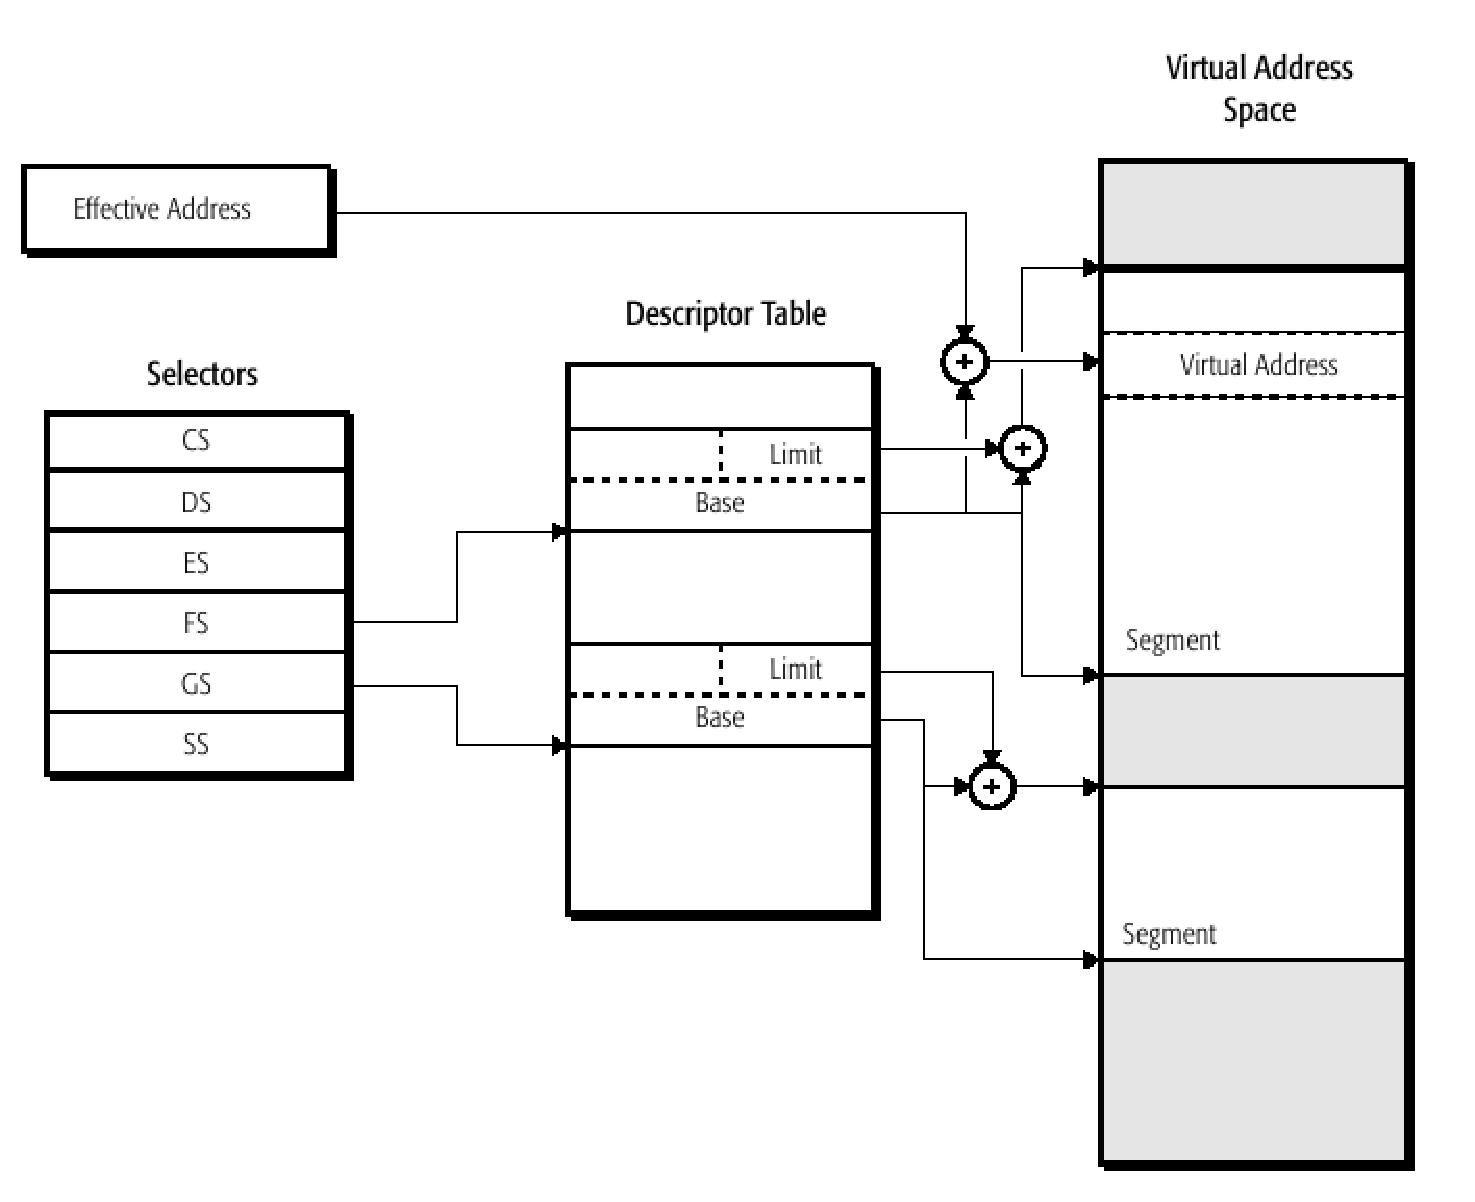
\includegraphics[scale=0.5]{./figures/segmentation.eps}
\caption{Segmented Memory Model}
\label{fig:segmentation.eps}
\end{figure}


The segmentation mechanism provides ten segment registers, each of which defines a single segment. Six of these registers (CS, DS, ES, FS, GS, and SS) define user segments. The remaining four segment registers (GDT, LDT, IDT, and TR) define system segments. The segment selector points toward a specific entry in descriptor table. This can be Global Descriptor Table (GDT) or Local Descriptor Table (LDT). The descriptor table entry base value plus the effective address which is the offset from base gives the virtual address. Effective address is calculated from the value stored in general purpose register and a displacement value encoded as part of instruction.

\subsection{PAGING}
Paging allows software and data to be relocated in physical address space using fixed-size blocks called physical pages. It translation uses a hierarchical data structure called a page-translation table to translate virtual pages into physical pages. Paging also provides protection as access to physical pages by lesser-privileged software can be restricted. ~\figurename~{\ref{fig:paging.eps}} shows an example of paged memory with three levels in the translation-table hierarchy. 




%\figurename{} 
\begin{figure}[H]
\centering
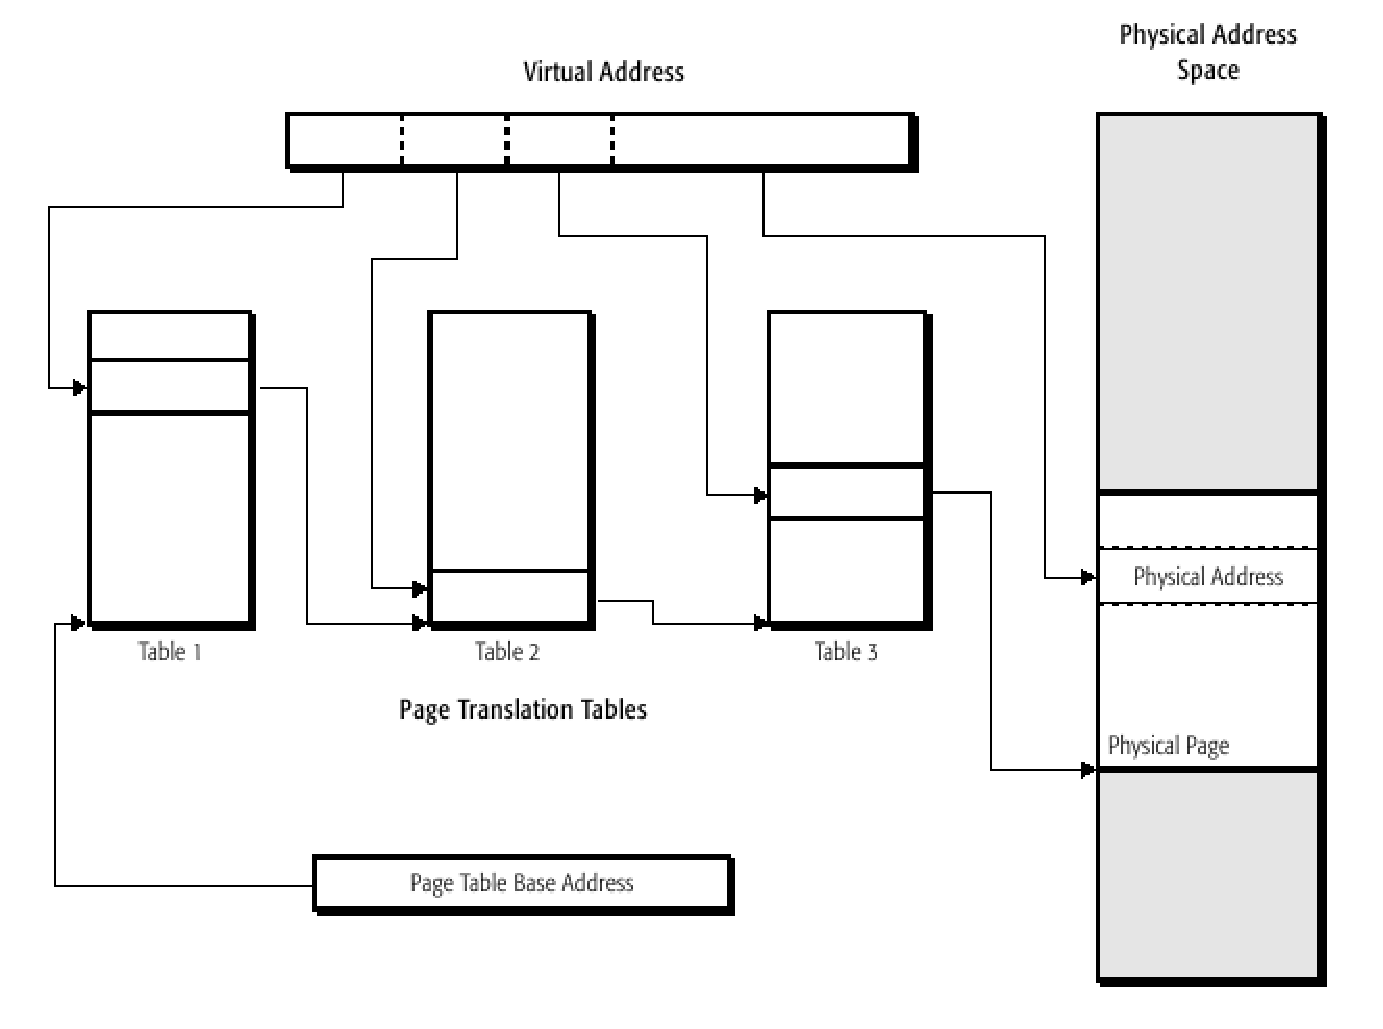
\includegraphics[scale=0.5]{./figures/paging.eps}
\caption{Paged Memory Model}
\label{fig:paging.eps}
\end{figure}



The number of levels in the translation-table hierarchy can be as few as one or as many as four, depending on the physical-page size and processor operating mode. Each table in the translation hierarchy is indexed by a portion of the virtual-address bits. The entry referenced by the table index contains a pointer to the base address of the next-lower level table in the translation hierarchy. Last page table entry plus the offset value from the virtual address (lsb bits), points toward the actual physical address.  


%%%%%%%%%%%%%%%%%%%%%%%%%%%%%%%%%%%%%% VERIFICATION ENVIRONMENT %%%%%%%%%%%%%%%%%%%%%%%%%%%%%%%%%%%%%%%%%%%%%%%
\newpage
\chapter{VERIFICATION ENVIRONMENT}
\label{chap:verification.tex}

\section {FUNCTIONAL VERIFICATION}

In SoC design methodology, the first step is to define the specifications. Once the system specifications are completed, design phase starts. The behavioral modeling of the design is done using hardware description languages like VHDL or Verilog HDL and in this stage the design is said to be Register Transfer Level (RTL). Such design could be partitioned to aid reusability, concurrent development and tool effectiveness. In general, reusable components of designs are packaged into components called Intellectual Property (IP). The RTL description of design is verified against functional specifications.  The system level verification is done to verify the RTL description against the intended functionality among other requirements such as timing, power and gate-count. 



Functional verification validates that the design meets the requirements. Test cases are created based on specifications. Various aspects of data and control flow are verified by passing information between external environments, communication with I/O devices,  software interactions etc. 
 
\section {VERIFICATION}

Most SoC verification concentrtes on verifying the processor cores and their interactions with SoC level IPs. At this level of abstraction, verification of interaction between the IPs and functional verification of top level modules are done.  Test conditions are written in x86 assembly and in some cases written in high level languages like C++. The intension of each test is to verify specific functionality of the design and ensure its validity. The test plans must to be in sync with the specifications of RTL design and are to be updated with new specification changes to ensure that it is efficient enough to deal with all possible corner cases and boundary conditions.

Tests are developed, so that they stimulate the design in a specific manner and compare outcome aganist expected outcome to assert accuracy of design behaviour. Ideally the design should be verified against all possible scenarios that could arise and once it passes all tests, it can be considered as completely verified. In case when a particular test fails, the verification engineer needs to find out the cause of failure with his understanding of design or verification aspect that led to the particular failure. This process of root causing a failure is called as a ``{\it debug}'' in verification. Once root-caused, the engineer then has to suggest appropriate changes to either design, verification or documentation to keep them in unison. 

There are many possible issues that can lead to a test failure. Each test defines conditions for pass and fail. A fail or pass is basically the outcome of a test run. There can be manly different causes for failures, with majority of them being:

\begin{description}
	\item[Self check fails]  In a self check failure, the program code running on the simulated processor is able to identify and report a failure. The program tests are written such that they evaluate the results, compare it with desired value and finally report fail or pass. 
	\item[Assertion/Checker fails] Assertion or checker fails are very common kind of failures and occur when a testbench component reports an unexpected behaviour of either the design or a verification component. In general, most checkers or assertions monitor particular design states during the simulation and report failure whenever monitored value deviates from the expected value. 
\end{description}

In general, a self check fail is caused when program execution deviates from the intended execution flow that was determined for the program under test. Hence the debug of a self check fail would require knowlege of the program under test and its intended execution flow. Without these knowledge, it would be a challenge to debug such fails. This project is aimed to improve debug of such self check fails.

%\subsection {DEVELOP TESTS}
%
%Tests for verifying all the features of the RTL are written in x86 assembly or in high level languages. These test plans are in sync with the specifications of RTL and are to be updated with new specification changes. Test cases should be efficient enough to deal with all possible []: 
%\begin{itemize}
%
%\item Corner cases
%\item Boundary conditions
%\item Design discontinuities
%\item Error conditions
%\item Exception/Interrupt handling
%
%\end {itemize}

\subsection {SELF CHECK FAILURE}

Processor tests are C/assembly program written to assert that the processor under test is indeed functioning as expected under that specific setup. These processor tests are designed such a way that they are capable of deciding if the processor execution results were successful. These tests are normally hand written by the verification engineer rather than randomly generated.  Hence such tests can string together specific stimulus of interest and determine pass or fail status on its own without relying on other verification components. Such tests are called as ``self~tests''.


%\figurename{} 
\begin{figure}[h]
\centering
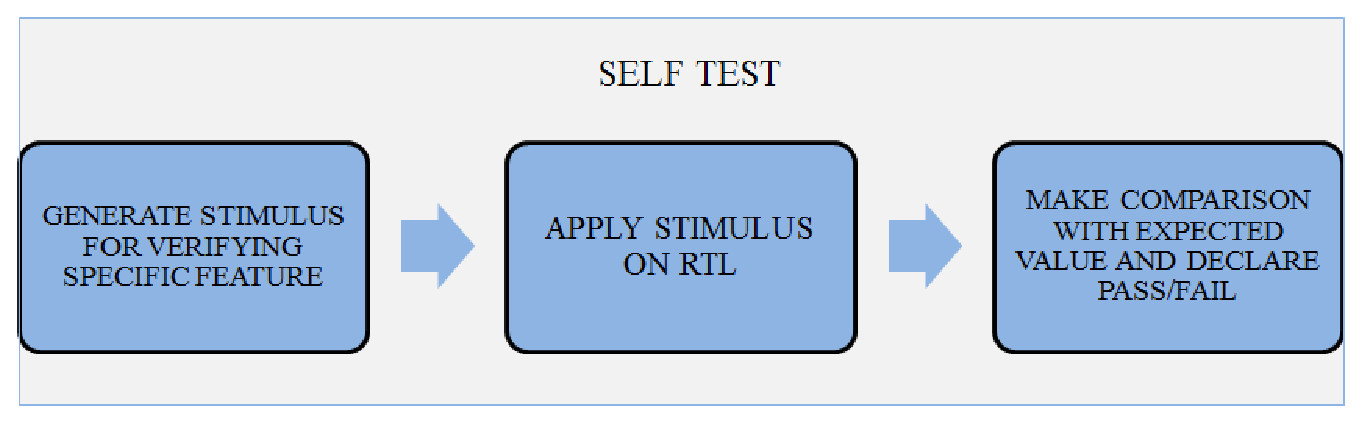
\includegraphics[scale=0.65]{./figures/selftest.ps}
\caption{Self-Test} 
\label{fig:selftest.ps}
\end{figure}

\figurename{\ref{fig:selftest.ps}} details the flow of a self~test. self~tests are a collection of x86 assembly language program. Tests are compiled by a script which calls an assembler followed by a linker. The final output being a linked binary image can be loaded and executed by the RTL model of DUT \nomenclature{DUT}{Design Under Test}. Stimulus is generated by the test and is applied to the DUT. Comparisons are done by the test itself after which pass/fail result is generated.



\section{DEBUGGING A SELF TEST FAILURE}

Self-tests report the occurrence of test case failure. Once this is available, next step is to analyze the reason for failure.  For this, a traceback from the point of failure to the point of error is required. 

A failure message indicates that the result is deviating from the desired value. This desired value can be understood from analysing the asm test code. But to understand at which point during execution the design deviated from the desired course, detailed information regarding execution flow as well as a reference flow which has the ideal values and status are required. In general, a reference flow could be established by the engineer after understanding and interpretting the test in its completeness.
 
To aid execution flow, RTL is simulated along with an instruction level reference simulator. The reference simulator is a software model which imitates the design functionally and executes same instructions in parallel with the RTL. This parallel simulation is also called as cosimulation and produces a log of processor activity.


\subsection {COSIMULATION}
The instruction level reference simulator (ILS) \nomenclature{ILS}{Instruction Level Simulator} is an x86/x86-64 compatible model, generally written in software languages such as {\it C++}. It models the processor in great detail including registers, caches and modes of operation. The test provides stimulus to both the RTL and reference models. An interface between RTL and reference model compares the states after each instruction retire and report any mismatch. 

The following section details the features and functions of simulator and interface. 



%\figurename{} 
\begin{figure}[h]
\centering
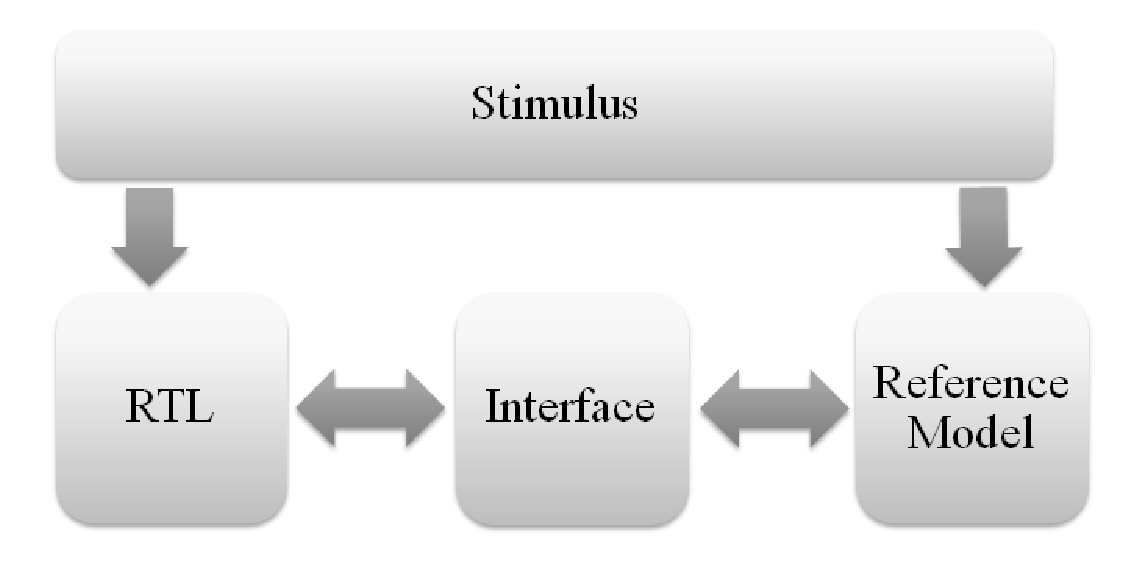
\includegraphics[scale=0.65]{./figures/interface.ps}
\caption{RTL-Reference Model Cosimulation} 
\label{fig:interface.ps}
\end{figure}



%\subsection {COMPARISON WITH REFERENCE MODULE}

%The RTL is simulated along with an instruction level reference simulator. This instruction level simulator is an x86/x86-64 programming model. It mainly models the register states and memory features and act as the ideal reference point to compare with. An interface between RTL and reference model compares the states after each instruction retire and report any mismatch. The following section details the features and functions of simulator and interface.

\subsubsection {INSTRUCTION LEVEL SIMULATOR}
The x86 instruction level simulator starts simulation after initializing the contents of its memory with linked binary image of the test. The ILS emulates the fetch/decode/execute algorithm of a scalar processor, producing an output log known as processor execution log. Each log entry describes the instruction, its results and any side effects it had on the processor state. The simulator models debug features, exceptions and interrupts as well as processor specific features. Supported processor states include x86 general purpose registers, flag registers, control registers, media registers, model specific registers as well as memory and I/O spaces. The simulator runs multithreaded code to simulate multiprocessor and multicore processor systems. 
The simulator runs in step with the RTL. Whenever an instruction or exception is retired in RTL that thread within the simulator is stepped-up and the processor states in the RTL and the simulator are compared. Difference detected in processor states are considered as a mismatch; difference in memory locations are also considered as mismatches and upon any mismatch, the cosimulation is terminated. At the end of the simulation when all threads stop executing, the memory states of RTL and the simulator are compared and any discrepancies are reported as memory mismatches.

\subsubsection {INTERFACE}
The interface between RTL and reference model keeps the ILS in step with RTL signal. It steps the ILS when an instruction in RTL simualtion has retired and then compares the results of execution between RTL and ILs. If the reference model is unable to model anything that is present in the RTL, the interface also re-synchronizes the ILS with the state obtained after execution of the RTL instruction.
Main functions of this interface includes
\begin{description}
	\item[Initialization] Initialize memory model, attach RTL signal and initialize some specific RTL signals.
	\item[Increment] Based on number of instruction retired per cycle, the interface informs ILS how many instructions to step.
	\item[Interrupt Handling] Interface informs ILS about pending interrupts
	\item[Comparing] Compares RTL and reference model registers; integer, FP, control and status word. Also reports any mismatches.
	\item[Interfacing with the memory model] Tell memory model what operations are seen by the RTL. 
\end{description}

\label{verif:exelog}
During the course of simulation, the ILS generates log files holding processor's program execution details. These are called ``\emph {processor execution log}''s. These log files will contain cycle by cycle information regarding register states, memory values, flags, threads etc. Basically all the comparison and debugging will require these information.

Once a failure is reported, simulation terminates and it would be required to be debugged. For root-causing the failure, verification engineer needs to trace through this processor execution log. Mismatches with reference model values provide information regarding the cause of failure.

Tracing through the log files is done manually. Data obtained from instruction simulation log and the assembled test files needs to be analyzed and correlated for debugging the failure. This is a very tedious effort consuming a lot of verification time. This is because of two main reasons:

\begin{enumerate}
	\item Relevant/required information is buried under a wealth of information
	\item Correlated information is spread across in different files
\end{enumerate}

As the design itself is very complex, these reasons makes manual tracing too time consuming. This will stretch the verification time and ultimately time-to-market.   


 

%%%%%%%%%%%%%%%%%%%%%%%%%%%%%%%%%%%%%% PROPOSED ENHANCMENT %%%%%%%%%%%%%%%%%%%%%%%%%%%%%%%%%%%%%%%%%%%%%%%
\newpage
\chapter{PROPOSED ENHANCEMENT}
\label{chap:enhancement.tex}

\section {VISUALIZING PROCESSOR EXECUTION}
Once the program is loaded in processor memory the execution starts. Generally modern microprocessors today adopt instruction level parallelism for high throughput. Micro-architectural like instruction pipeline, superscalar execution, register renaming, speculative execution, branch prediction etc. are employed in order to exploit instruction level parallelism [].  \\
An execution log file captures all the information regarding the processor state and activity during the execution of a code. Each entry in the log file will have the following information:
\begin{itemize}
	\item The instruction number and opcode
	\item Thread Id (in multi-core and multi-processor)
	\item Memory read/write information
	\item Code read/write
	\item I/O read or write
	\item Interrupt and exception information
	\item Branch Target
	\item Paging info
	\item Flag values
	\item Register updates made
\end{itemize}
On the onset of a simulation failure, these information are very vital. For understanding how execution log information helps in debugging failure let us consider two test scenarios.

\section {CASE STUDY}

\subsection {TEST A}
Consider an assembly code of testing a memory module. The test writes a value into a memory location. The data is later read from the same location and read data value is compared with the original value written into the location. The test flags a fail of pass based on the comparison.\\

\IncMargin{1em}
\begin{algorithm}[H]
\DontPrintSemicolon
\SetKwInOut{Input}{Input}\SetKwInOut{Output}{Output}

\Input{$data$, $address$}
\Output{Test result: $pass$ or $fail$}
\BlankLine
Initialization: Select memory bank by setting $Control Register$ \;

	$Reg A \longleftarrow data$\;
	$Reg B \longleftarrow address$\;

	Memory $[Reg B] \longleftarrow Reg A $\;

	$Reg C \longleftarrow data$\;

	$Reg D \longleftarrow$	Memory $[Reg B]$\; 

\eIf{$Reg C == Reg D$}{
report $pass$
}{
report $fail$
}

\caption{Memory Read-Write}
\end{algorithm}\DecMargin{1em}

\vspace{2cm}
The test verifies write/read from a memory location. Ideally the values written to the memory location should match the value read from the memory and test completes with a pass. Now consider a situation where the comparison fails. This can happen due to many reasons. Following are a few scenarios which can lead to a failure:
\begin{itemize}
\item [Case 1]: If due to some external process the control bit for bank selection is changed in between the execution, the data read will be from wrong memory location leading to failure.

\item [Case 2]: If the address value is invalid. This can happen when the test generates a random address value for storing the data and this value might not exist in the current selected memory bank range.

\item [Case 3]:  If the register chosen is read only. This will cause the wrong data to be updated into the memory and comparison fails.
\end{itemize}

\subsubsection{ANALYSIS}
Consider Case 1. The memory bank selected should stay same throughout the program execution. This change in memory bank will cause the read operation to take value from wrong memory block. This will lead to self-test failure. \\
 Now to understand when and where the actual error occurred, we need to keep track of the control register value and see where the value changed from expected value. For this we need to start tracing the values from the point of failure. \\

Case 2. Each memory block has a fixed size. The base value will be selected on setting the control bit. The offset value is provided by the test. A valid address value will be within the range of memory block that is between the lowest and highest offset. Any attempt to access a value which doesn't lie within this range will evidently lead to an error.\\
If such a situation occurs, the user needs to be aware of the particularities of each memory write operation. Details on instance of memory write, actual physical as well as logical address value, instruction cycle number etc are required to figure out if this was the cause of test failure.\\
Case 3.  Certain bits of some specific registers are set as read-only. Suppose a case where a 32 bit register A has its lower byte set as read-only and has the value XXXXXX00h. If the test is trying to set this register to a certain value, for example FFFFFFFFh, chances are that the value that is actually set might not be a FFFFFFFFh but some other value possibly FFFFFF00h. 
To catch such an error, the verification engineer needs to know the value stored in each register used during test at all cycle.






 

%%%%%%%%%%%%%%%%%%%%%%%%%%%%%%%%%%%%%% INTERFACE IMPLEMENTATION %%%%%%%%%%%%%%%%%%%%%%%%%%%%%%%%%%%%%%%%%%%%%%%
\newpage
\chapter{INTERFACE IMPLEMENTATION}
\label{chap:GUI_impl.tex}
The GUI provides user friendly and easy data navigation which will reduce debug efforts. All relevant processor execution log information and asm test details are provided to the user through a web interface. The interface uses data visualization JavaScript features to develop graphical representation of the log information. Features of the GUI are designed such that, traversing through the log information and comparison with the asm list file lines are made easy.  Major processor operations are categorized and extracted to have a clear view of processor actions.  From analysis done in Chapter 3, the following sets of features are expected to help the user and are our main design objective while implementing the interface:
\begin{itemize}

\item[-] Visualizing the processor execution flow in each thread
\item[-] Information regarding each Memory write/read, I/O write/read, Branching etc
\item[-] Interrupt and exception happening during execution
\item[-] Easy traversal to the asm instruction line.
\item[-] Register values at each instances
\item[-] Comparison of register values between two cycles
\item[-] All the cycle information provided by the cycle in execution log for detailed reference.
\end{itemize}
Once the simulation is completed and failure is reported the debug phase starts. This is where the role of GUI comes. From the vast information provided by the logs and test files, interfaces have to capture and represent relevant information to the user. The following section details the implementation and features of the proposed GUI. 

\section {INTERFACE IMPLEMENTATION}
GUI is implemented as a HTML web page. Each test case will have its one set of log files and asm list files. The interfaces implementation starts by taking these files are input.  Two programming languages are used for implementation:
\begin{itemize}
\item[-] Python Script for data extraction and correlating related information.
\item[-] JavaScript for designing the interface features and user interaction.
\end{itemize}
Figure x shows the implementation of GUI.

\addtocontents{toc}{\protect\setcounter{tocdepth}{2}}
%\figurename{} 
\begin{figure}[H]
\centering
\includegraphics[width=5.5in]{./figures/GUI_impl.eps}
\caption{GUI Implementation} 
\label{fig:GUI_impl.eps}
\end{figure}

 Major implementation steps
\begin{itemize}
\item[-] The asm list file and processor execution file informations are extracted by python script.
\item[-] A top level python program will manipulate these information are convert it to JavaScript objects. 
\item[-] JavaScript code for developing user interactive features is written.
\item[-] The top level python program will combine the data extracted and javascriot code and generate a single HTML page. 
\end{itemize}
Inputs to the implementation are Execution log file and Asm list files. To develop the GUI the user has to execute the top level python script with these two files as input argument. The script will generate an output file which is the interface web page. Major processes involved in implementation are detailed below. 


\subsection {EXTRACTING ASM FILE INFORMATION}
The test code is written in x-86 assembly language. While debugging the instructions and values in the asm file is the expected action or value.  Each cycle in processor execution log corresponds to a particular code line in asm. However the asm code written by the verification engineer is the unscheduled code without any memory address details. For cycle comparison with execution log, the asm test file is complied first.  This is done by an assembler. Figure x shows how an asm test file is converted to a list file which hold an expanded, loop unrolled, scheduled code with memory details included.  
%\figurename{} 
%\figurename{} 
\begin{figure}[H]
\centering
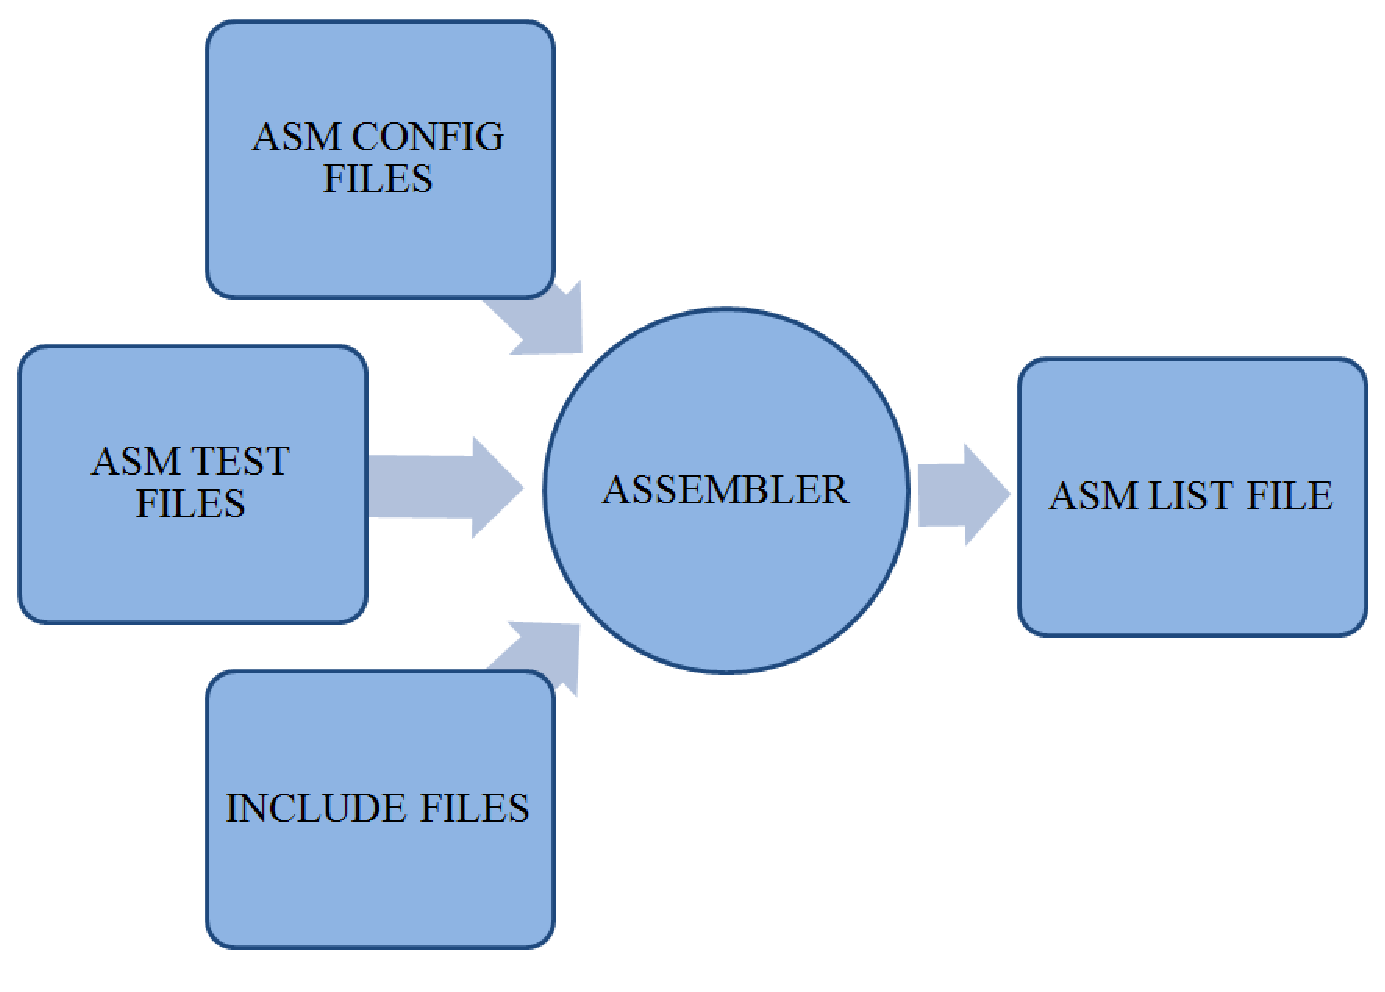
\includegraphics[width=3.5in]{./figures/asm.eps}
\caption{Assembler}
\end{figure}


A 64-bit assembler assembles asm test file, configuration file (that define the random operands, segmentation, gdt, ldt, page tables, etc,) and the include files together to generate an assembly list file [1].
\begin{figure}[H]
\centering
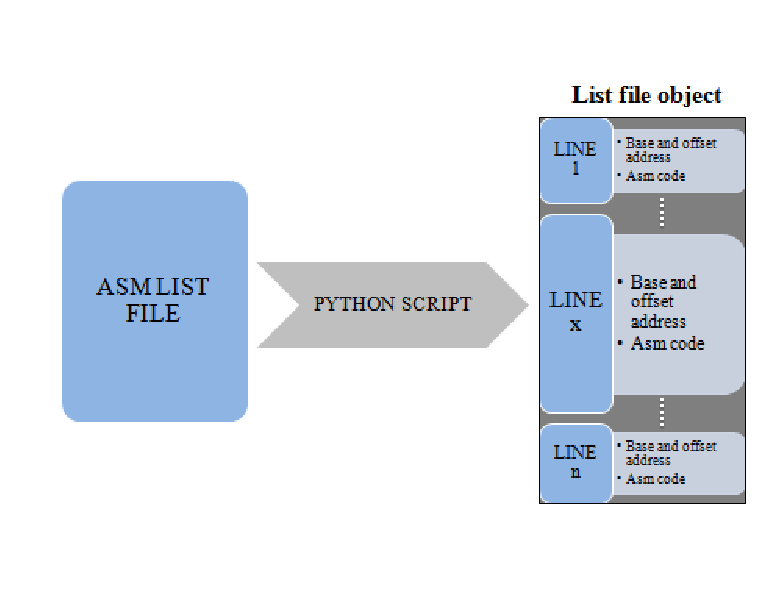
\includegraphics[width=4.5in]{./figures/list.eps}
\caption{Asm List File Extraction}
\end{figure}
List file holds details of instructions; opcodes and operand, linear address, module/register configuration details etc. For the purpose of correlating informations, a python script will extract relevant information corresponding to each instruction line in the list file.  For each line number the script will create an object which will have the following parameters.
\begin{itemize}
	\item[-] Base and offset address value
	\item[-] Instruction line number
	\item[-] The assembly code
\end{itemize}

Figure x shows how python script will read the input asm list file and generate a data structure of list objects corresponding to each line. 

\subsection {EXTRACTING EXECUTION LOG INFORMATION}
The second input to the implementation is the execution log file. As explained in previous chapters, debugging require detail traversal through this log file as it holds instruction by instruction execution details which include register states, thread details, flags information etc and other data which help in tracing out the cause of failure. 

All details given in the log file in reference to each cycle are to be extracted. The python code will extract this as well are generate a data base of log file object corresponding to each cycle of execution. These are classes with properties corresponding to major operations and register values. Each thread will have a separate handle with objects corresponding to each cycle of operation in that thread. Figure x shows how the script will read the input execution log file and generate log file objects.
Each object in the log file will have the following properties associated with it:

\begin{itemize}
 \item[-] Thread number
 \item[-]  Mode of operation
 \item[-]  Cycle number
 \item[-]  Linear address
 \item[-]  Memory write, Memory read, I/O write/read, Code read
 \item[-]  Branch target (linear address)
 \item[-]  Registers updated with new value
\end{itemize}


\subsection {Correlating asm file objects and log file objects}

Once both the input files are processed, next step is correlating the asm file object and log file object. The top level python script will combine these these to in pairs based on the address mapping. As x86 architecture follows segmented memory model along with paging, address translation is required for generating the linear/physical address [2]. For each object in the generated list file class, calculate the linear address as follows:
\\
\centerline{Linear address = Base address + Offset value}
\\
For each object in the log file class, find the corresponding list file object based on the linear address value and combine the objects.
\IncMargin{1em}
\begin{algorithm}[H]
\DontPrintSemicolon
\SetKwInOut{Input}{Input}\SetKwInOut{Output}{Output}

\Input{list file objects$\rightarrow listObj[]$, log file object$\rightarrow logObj[]$}
\Output{Test result: $pass$ or $fail$}
\BlankLine
Start: \;
For {each object $list$ in listObj}{\;
		list.address = list.Base + list.Offset\;
	}
For {each object $log$ in logObj}{\;
	set count = 0\;
	For {each object $list$ in listObj}{\;
	 \If{$log.address == list.address$}{
		Add $list.property \rightarrow log.property$\;
		count = 1;
		break loop\;
	}
	}
	\If{count == 0}{
	assert: $"no address match"$
	}
}
End \;
\caption{Memory Read-Write}
\end{algorithm}\DecMargin{1em}

\vspace{2cm}
Input: list file objects, log file objects
Start:
For each object in list file class do
	listObj.address = listObj.Base + listObj.Offset
end

For each object in log Class do
	For each object in list file class
		If logObject.address == listObj.Address
			Add listObj properties to logObject
			Break loop;
	End
	End
End
Now we have a set of objects that hold log details and are linked to corresponding asm file line. Once this stage is completed we have completed all the data extraction and next phase is building the interface.

\subsection {DEVELOP THE INTERFACE}

The final step is developing the interface. As the GUI is web based, layout design is done using HTML (Hyper Text Markup Language). However for providing interactive features to the user a much more powerful language is need along with HTML and we use JavaScript.

\emph {\bf JavaScript (JS)} is an interpreted computer programming language. It is  implemented as part of web browsers so that client-side scripts could interact with the user, control the browser, communicate asynchronously, and alter the document content that was displayed. It is a multi-paradigm language, supporting object-oriented, imperative, and functional programming styles.

In addition a style sheet language called CSS (Cascading Style Sheets) is used for describing the presentation semantics (the look and formatting) of the interface page written in HTML.

 

%%%%%%%%%%%%%%%%%%%%%%%%%%%%%%%%%%%%%%% GUI FEATURES %%%%%%%%%%%%%%%%%%%%%%%%%%%%%%%%%%%%%%%%%%%%%%%
%\newpage
%\chapter{GUI FEATURES}
\label{chap:GUI_features.tex}
%\addtocontents{toc}{\protect\setcounter{tocdepth}{0}}

The master Python script reads all the extracted information from the log files and the list files. This script finally generates a single HTML page for the interface. The interface mainly features:


\section {EXECUTION FLOW GRAPH}

Main feature of the web page is the graph showing the execution flow of the code. Here asm list file line numbers are plotted against the cycle during which it is executed. All the active threads have different graphs which are tabbed. Hovering the mouse over any point on the graph will display x and y axis values. 
 
This zoom enabled data graphs also provides onclick selection of specific operations e.g: Branching, Memory Write, Memory Read, Code Read etc, which will display the instances of selected operation. Each operation is distinguished by its color.   


\section {REGISTER WATCH WINDOW}

Register window capture and display updated register values at a specific instance. Each thread holds its own copy of registers/flags. A selection of point on the execution flow graph will update the register window with values at that instant in the selected thread. Values of following registers and flags are provided to the user:

\begin{itemize}
	\item[-] 64 bit general purpose registers (RAX, RBX, RCX etc)
	\item[-] RFLAG (64 bit)
	\item[-] Instruction Pointer (RIP)
	\item[-] Stack Pointer (RSP)
\end{itemize}

Another feature provided by register window is comparison between register values at two different instances that is between a reference point set by Set Marker button and current selection. 


\section {INSTRUCTION WINDOW}

Instruction window give the asm file lines. A selection in execution graph will be reflected in this window by highlighting the asm file instruction corresponding to the selected point. Also the context of the selected line that is its preceding and succeeding instructions are also available in this window.

\section {EXECUTION LOG WINDOW}

In addition to the instruction and register information, all the processor execution log information regarding the selected instruction is also provided through execution log window.

\section{SET AND CLEAR MARKER}
These two options allow setting or removing a reference point with which current register values are compared against.

 


%%%%%%%%%%%%%%%%%%%%%%%%%%%%%%%%%%%%%% RESULT: GUI %%%%%%%%%%%%%%%%%%%%%%%%%%%%%%%%%%%%%%%%%%%%%%%
\newpage
\chapter{RESULTS: GRAPHIC USER INTERFACE}
\label{chap:GUI_results.tex}
\addtocontents{toc}{\protect\setcounter{tocdepth}{1}}
The final GUI is a HTML page generated by the master phyton script. This file is generated by running master script with the asm list files and execution log files as input. The generated .html or .htm file can be viewed by any standard web browser like Internet Explorer, Firefox etc that support JavaScript. As this is just like any other html page with out any dependences, the user can access the page from web as a stand-alone file with out requiring the list files and log files. 
The following figures shows various windows of final GUI.
\section {EXECUTION FLOW GRAPH}
%\figurename{} 
\begin{figure}[H]
\centering
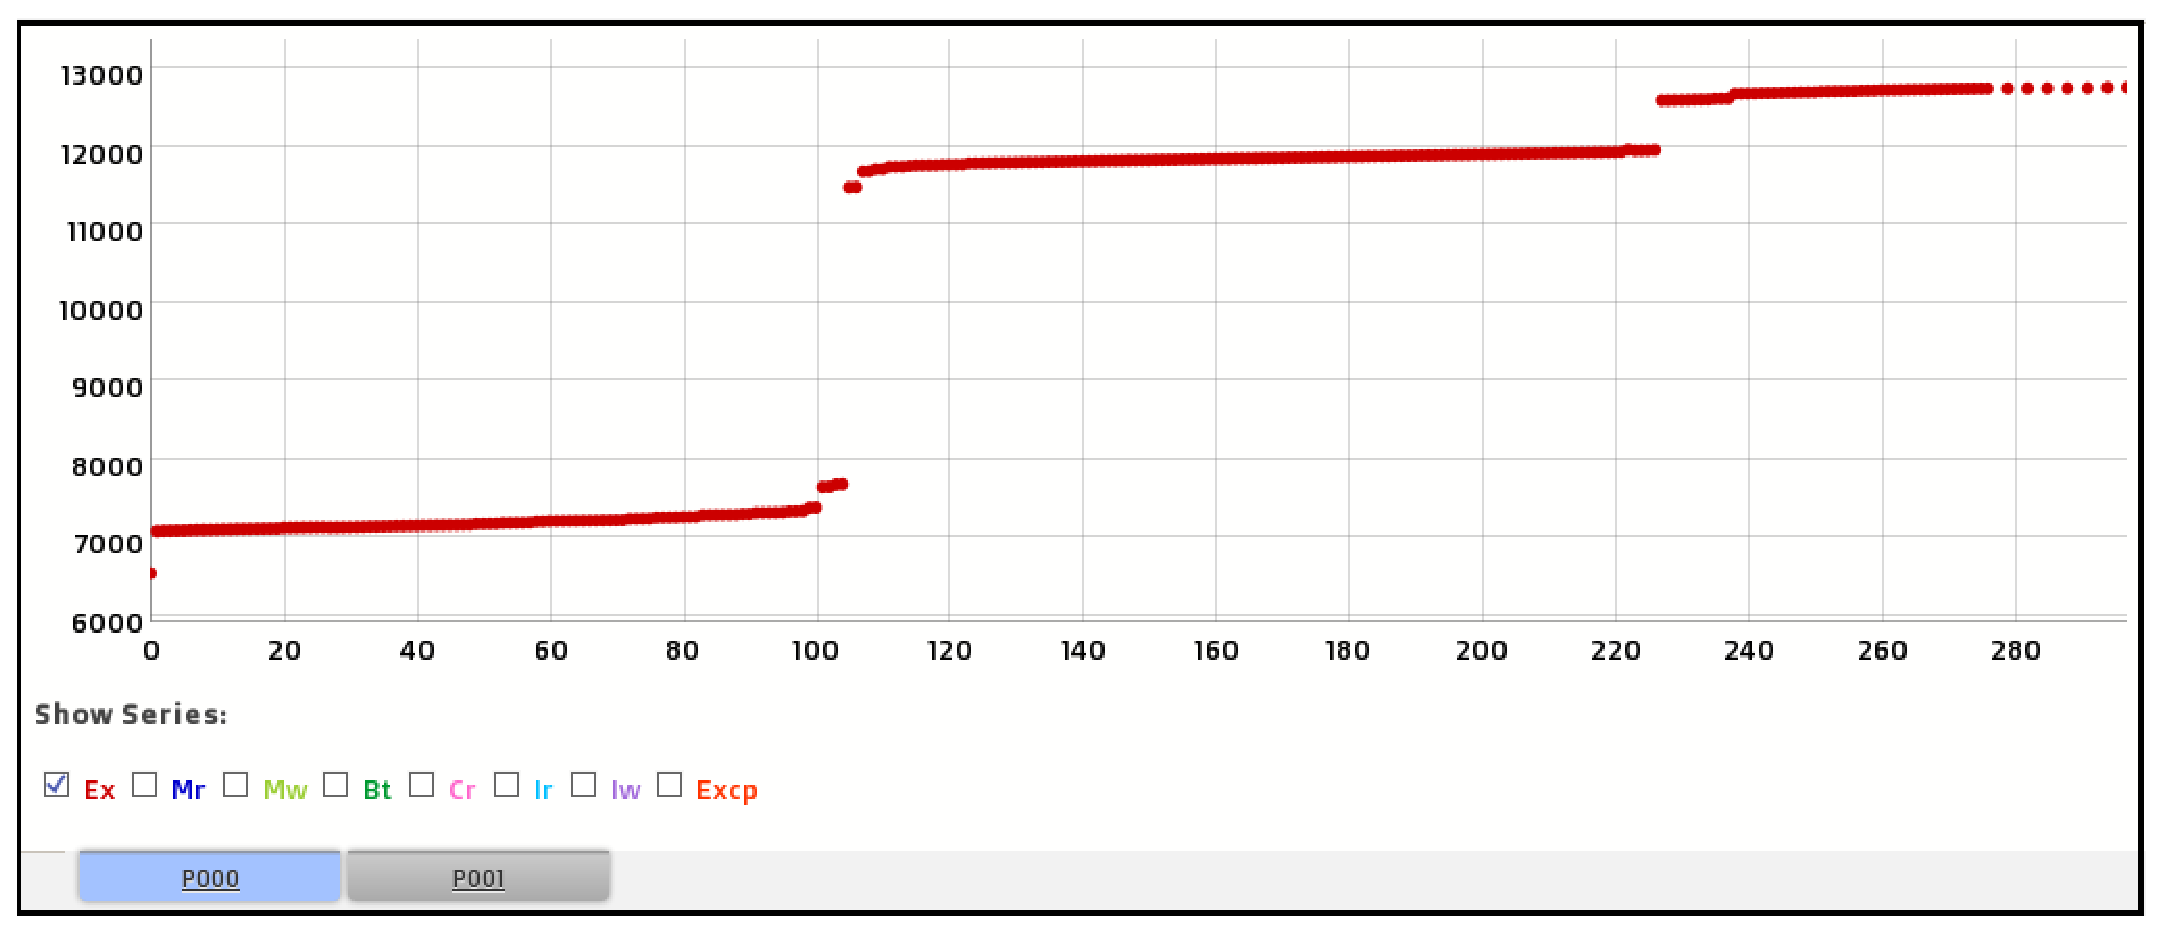
\includegraphics[width=6in]{./figures/gui_graph1.eps}
\caption{Execution Flow Graph}
\label{fig:gui_graph1.eps}
\end{figure}
%\end{tabular}
%\figurename{} 

~\figurename{~\ref{fig:gui_graph1.eps}}shows the main execution flow graph for selected active thread.  
\begin{figure}[H]
\centering
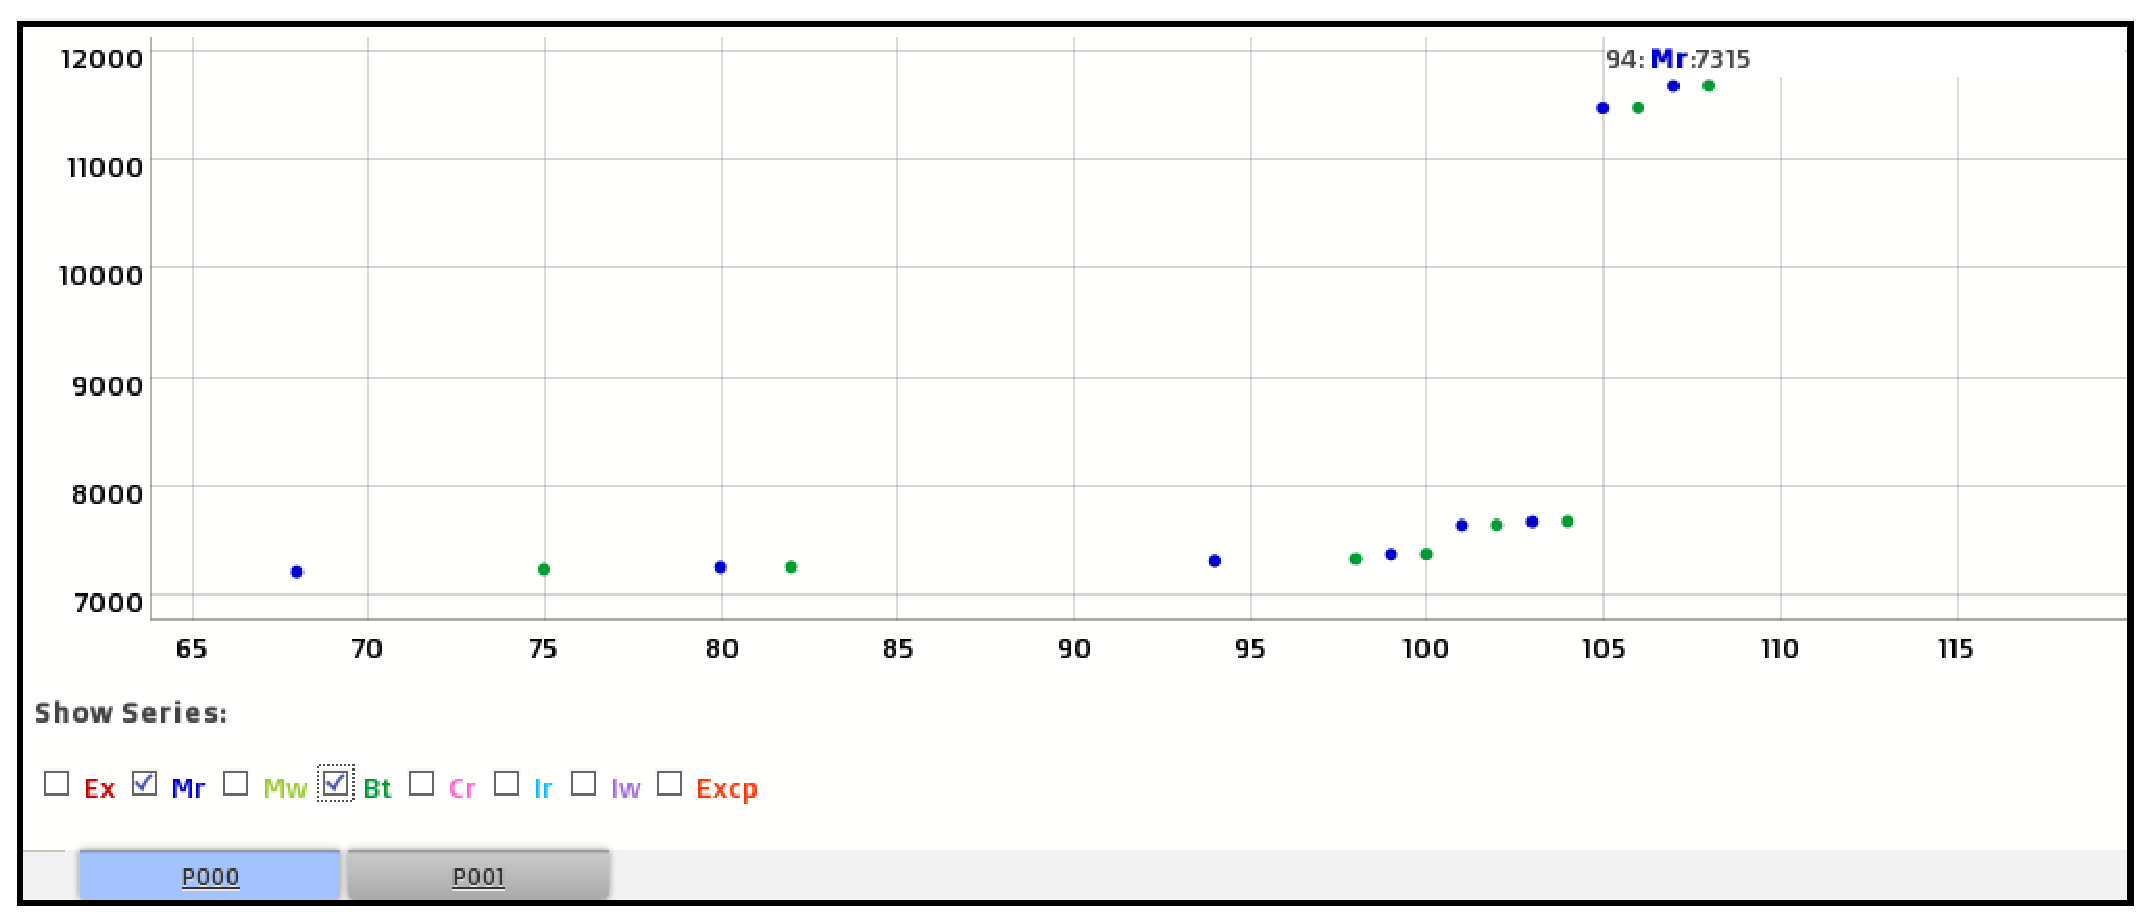
\includegraphics[width=6in]{./figures/gui_graph2.eps}
\caption{Execution Graph With Branching and Memory Writes}
\label{fig:gui_graph2.eps}
\end{figure}
%\end{tabular}
%\figurename{} 

~\figurename{~\ref{fig:gui_graph2.eps}} shows only memory write and branch operation happening in the selected thread.
\section {REGISTER WATCH WINDOW}
\begin{figure}[H]
\centering
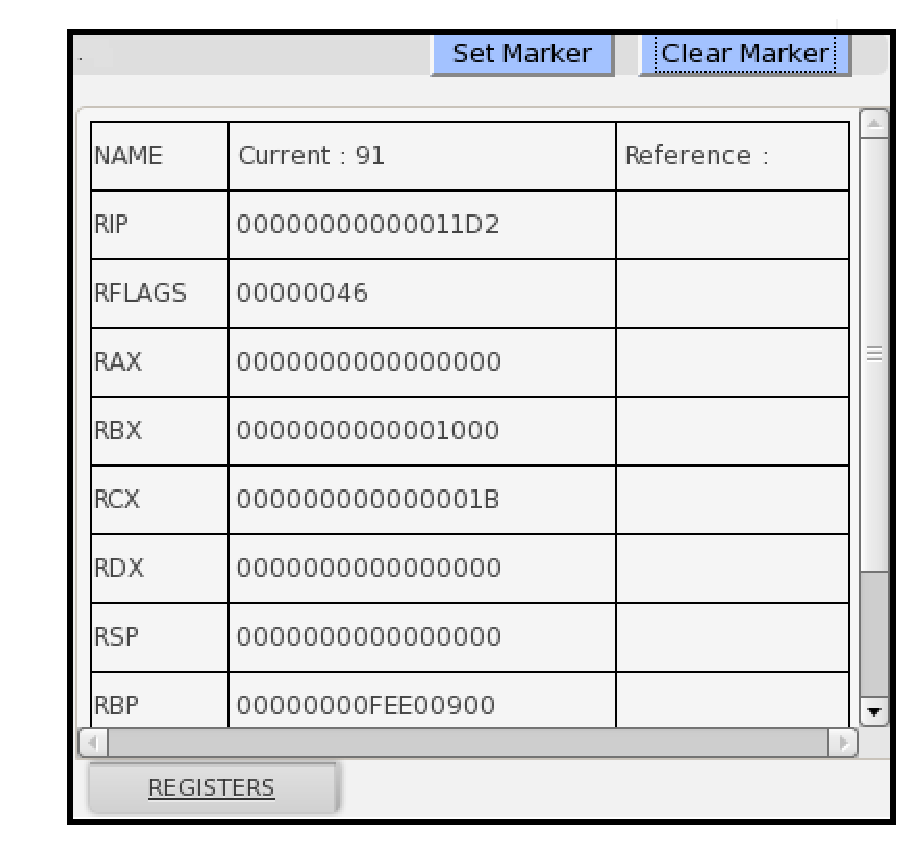
\includegraphics[width=4in, height=2in]{./figures/gui_reg1.eps}
\caption{Register Watch Window}
\label{fig:gui_reg1.eps}
\end{figure}
~\figurename{~\ref{fig:gui_reg1.eps}} shows register window showing updated register values of current selection.
%\end{tabular}
\begin{figure}[H]
\centering
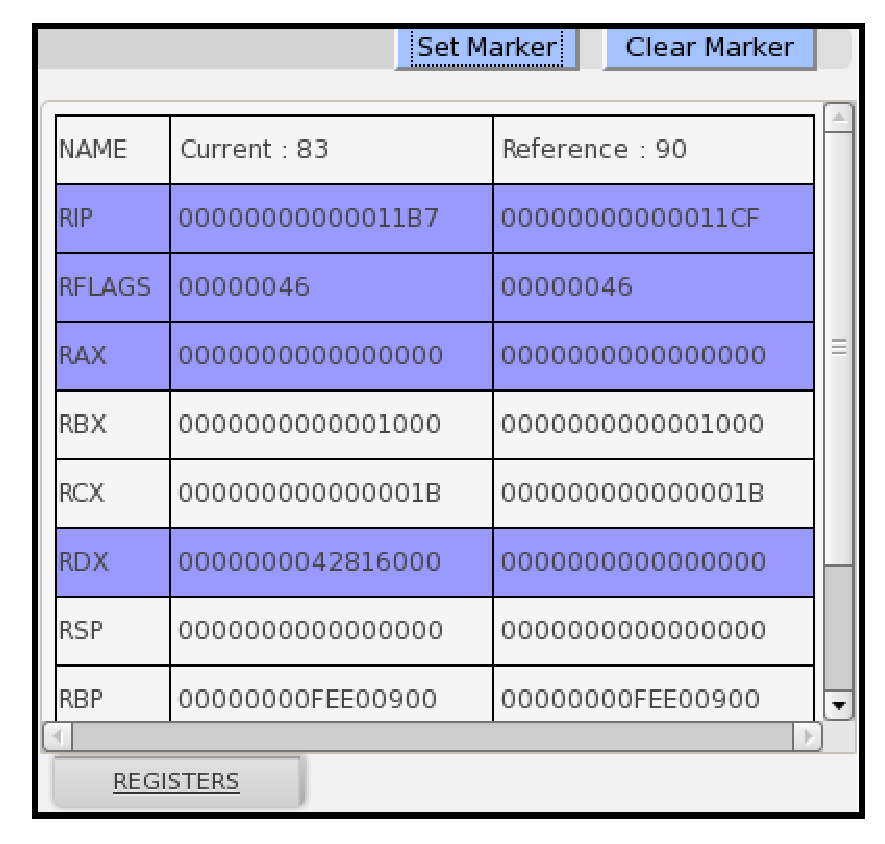
\includegraphics[width=4in, height=2in]{./figures/gui_reg2.eps}
\caption{Register Value Comparison}
\label{fig:gui_reg2.eps}
\end{figure}
%\end{tabular}
~\figurename{~\ref{fig:gui_reg2.eps}} shows the comparison of register states at two different points. Differences are highlighted.
\section {INSTRUCTION WINDOW}
\begin{figure}[H]
\centering
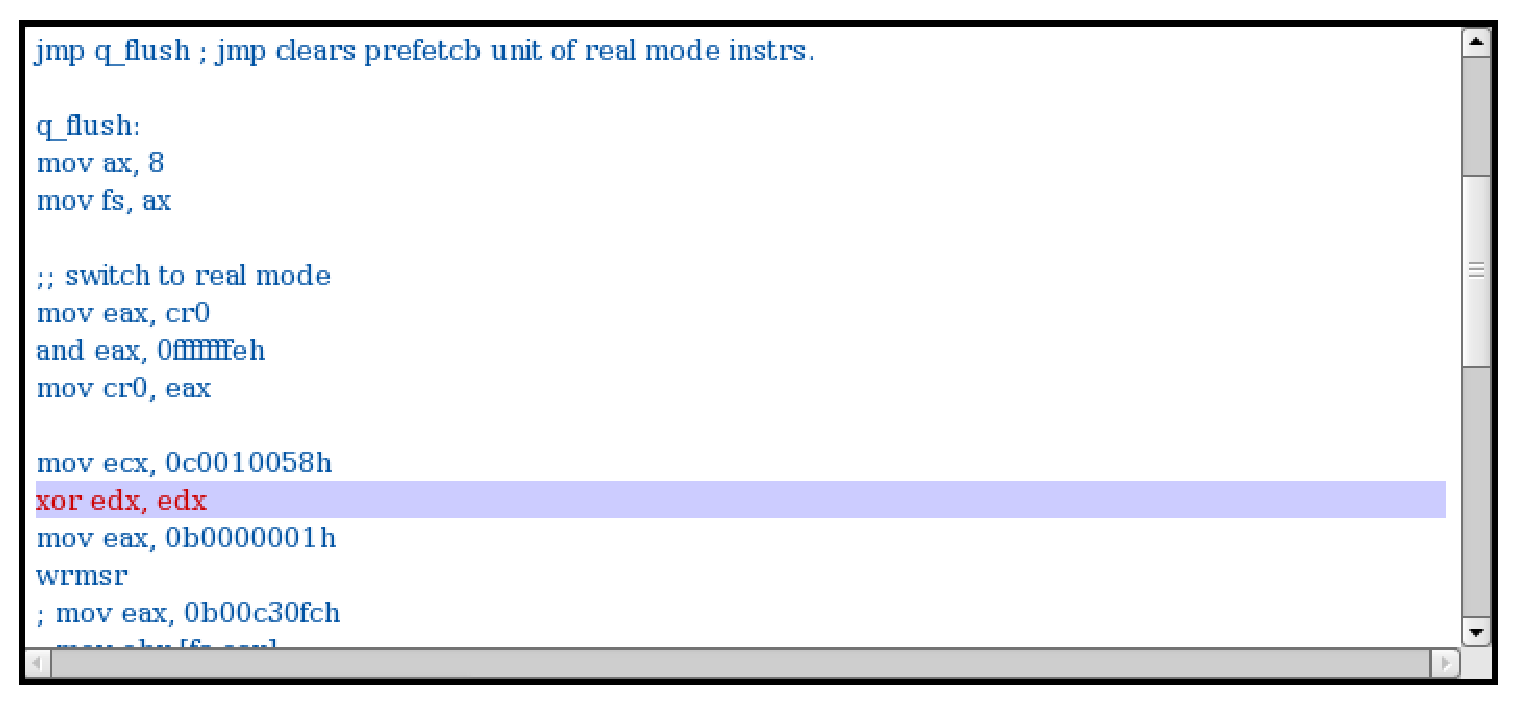
\includegraphics[width=5in, height=3in]{./figures/gui_asm.eps}
\caption{Instruction Window}
\label{fig:gui_asm.eps}
\end{figure}
%\end{tabular}
~\figurename{~\ref{fig:gui_asm.eps}} shows the instruction window which highlights the current selection and also display the context of selected instruction.




































 

%%%%%%%%%%%%%%%%%%%%%%%%%%%%%%%%%%%%%% CONCLUSION %%%%%%%%%%%%%%%%%%%%%%%%%%%%%%%%%%%%%%%%%%%%%%%
\newpage
\chapter{CONCLUSION}
\label{chap:GUI_conclusion}

An interactive off-line graphical user interface was designed and developed. The interface is completely web based and achieves primary goals of off-line debug. The interface contains all relevant information from processor execution log and assembly list files commonly needed for debug. Further debug if required, could be accomplised by traditional methods.

Execution graph helps in analysis of various operations like branching, exception, read/write etc and also to navigate through processor execution with ease. The graph presents thread-wise informations seperately, making tracing and navigation easy. The register window provides comparison between registers and flag values at two different execution cycle which helps in tracing a wrong value written into register or flag. Instruction window and execution log window provide common information necessary for debug.

\paragraph{Potential for future work:} The project demonstrates that web-based technologies like {\it html, JavaScript, CSS} are effective in enabling interactive remote debug. There is larger scope for this work in future as it gets adopted by different teams. New debug features like break points, cache containers, address filters among others could be introduced when in demand.




%%%%%%%%%%%%%%%%%%%%%%%%%%%%%%%%%%%%%% PART II : GATESIM %%%%%%%%%%%%%%%%%%%%%%%%%%%%%%%%%%%%%%%%%%%%%%%%%%
\part{}

%%%%%%%%%%%%%%%%%%%%%%%%%%%%%%%%%%%%%% INTRODUCTION %%%%%%%%%%%%%%%%%%%%%%%%%%%%%%%%%%%%%%%%%%%%%%%
\newpage
\chapter{INTRODUCTION}
%\section{Background}
%\section{Purpose/Motivation}
%\section{Approach}
%\section{Main Contributions}
%\section{Organization of thesis}

Functional verification of a design is the task of verifying that the logic design conforms to specifications and ensures functional correctness of the design.  With the rapid increase in design complexity and size, this phase of circuit design has become the most crucial and resource-intensive. It is widely accepted that more than 70 percent of design efforts is spend on verification and with the advancement in silicon technology and adoption of complex SoC designs; this situation is only projected to get worse in future~\citep{phd:zhang}. 

Verification is done at different abstraction levels. Two main abstraction levels from verification point of view are RTL and gate-level~\citep{phd:zhang}. RTL enables relatively easier management of complex designs and has less verification time requirements compared to gate or netlist-level. However it cannot eliminate the need for verification at netlist-level as each level is required for specific type of verification. While RTL verification is apt for functional validation or architectural analysis, more detailed analysis like timing, power etc require detailed models of lower levels. Another important challenge is ensuring the functional equality of models at different abstraction level.  

 Traditionally simulation based verification has be used as the primary approach for verification at both RTL as well as gate-level.  But with very complex designs, this approach has become inefficient in finding subtle design bugs. Also at gate-level, simulation based verification takes rather too much time that an exhaustive verification is impossible. On the other hand, formal verification tools have gained popularity since it can mathematically prove or disprove the design validity. These mathematical methods require less manual effort than simulation based verification and hence a lot faster. However these mathematical models cannot comprehend all kind of complexities that could occur in the design and it is very much clear that this alone can solve all issues. Rather a mix of simulation and formal verification methods are practiced to ensure all corner cases are covered. 


\section{GATE-LEVEL SIMULATION}

Gate-Level Simulation (also called as Gatesims) still play crucial role in verification, in spite of advancement in formal and static verification techniques like LEC \nomenclature{LEC}{Logic Equivalence Check} and STA \nomenclature{STA}{Static Timing Analysis}~\citep{ieee:segev:2004}.   When having to verify with Gatesim one has to start planning early, as it has to pass through various stages before sign off. The setup for gate-level simulation starts right after the prelim netlist is available and will continue till final post layout netlist.  

Even though Gatesims help in finding many issues related to timing and power, it is considered as a ``{\it necessary evil}'' by engineers. This is mainly because gate-level simulation is inherently very slow. It is also hard to find the optimal list of test cases to effectively utilize Gatesims. Debugging is also very tedious at gate-level and combined with the long run time, makes turn-around for debug long and ultimately affects time-to-market of the product.

Various approaches have been adopted over the years for gate-level simulation with each method trying to improve simulation performance and ease of debug. Since generally netlists are ``{\it Verilog}'' based, test environments used for RTL verification could be reused for netlist verification by replacing RTL with netlist as appropriate. It should also be possible to have the test vectors generated for RTL simulation used as stimulus for netlist simulation. Such application of test vectors can be done either by having the RTL be simulated in parallel with Gatesim or by applying captured test vectors from RTL simulation onto netlist simulation. The first method of stimulus application is called a cosimulation approach and the second is called a dual-simulation or sim after sim approach. Each method has its own set of pros and cons. Simulation time, design complexity, memory, ease of debug, testbench complexity tradeoffs are considered while choosing any particular method for Gatesims in a project. This thesis analyzes the advantage and disadvantage of past and present Gatesim methodologies and  proposes a new improved sim after sim or dual-simulation approach to Gatesims. 



\section{ORGANIZATION OF THE THESIS}
The organization of this project report is as follows:\\
\noindent 
{\bf Chapter}~\ref{chap:gate_intro.tex} -{\it Gate-Level Simulation} explains the relevance, advantages and limitations of gate-level simulations.\\
{\bf Chapter}~\ref{chap:methodologies.tex} -{\it Gatesim Methodologies} briefly explains various approaches used for Gatesims, their advantages and disadvantages.\\
{\bf Chapter}~\ref{chap:dualsim.tex} -{\it Improved Dual-Sim Approach To Gatesim} describes the implementation and flow of proposed dual-sim approach .\\
{\bf Chapter}~\ref{chap:results.tex} -{\it Results} gives comparison of simulation performances and memory utilization of current and proposed approaches.\\
%{\bf Chapter}~\ref{chap:GUI_results.tex} show the GUI windows and    .\\
{\bf Chapter}~\ref{chap:conclusion} discusses the various conclusion drawn from the results and the scope for future work.
 

%%%%%%%%%%%%%%%%%%%%%%%%%%%%%%%%%%%%%% GATE LEVEL SIMULATION %%%%%%%%%%%%%%%%%%%%%%%%%%%%%%%%%%%%%%%%%%%%%%%
\newpage
\chapter{GATE LEVEL SIMULATION}
\label{chap:gate_intro.tex}

In a typical VLSI design flow, the first step is creating an RTL level model of the design and writing the behavioral test bench for functional verification of this model. Once the functional RTL verification is completed, the next stage is design synthesis. During synthesis RTL is turned into a design implementation in terms of logic gates. Synthesis is mostly an automated process using a “{\it synthesizer}” tool that converts RTL-level design source code into gate-level netlist file.

 The netlist out of synthesis tool is then fed into layout tool which produces the layout of the design. During this process modifications are done on netlist but it remains functionally equal to its corresponding RTL. Netlist written by layout tool after layout has been done is called a post layout netlist.~\figurename{~\ref{fig:gatesim.eps}} shows where Gatesim comes in design flow.

%\figurename{} 
\begin{figure}[H]
\centering
\includegraphics[width=3.5in]{./figures/gatesim.eps}
\caption{Design Flow}
\label{fig:gatesim.eps}
\end{figure}
Gate Level Simulation or Gatesim focuses on verifying the post layout netlist of a module. Originally developed for verifying the functional correctness of chip netlist when formal tool were not available; Gatesims are currently used to complement and cover gaps left by formal flow. 


\section {NEED FOR GATESIM}
Gatesims are generally used for verifying the following. 
\begin{itemize}
	\item[-]To check if power-up, reset operation and initialization of the design are proper.
	\item[-]The RTL written is synthesizable.
	\item[-]DFT structures that are absent in RTL and are added during or after synthesis, they are not checked by simulation.
	\item[-]The netlist passes all the critical test scenarios.
	\item[-]Any un-initialized outputs.
	\item[-]Low-power structures that are absent in RTL and added later during synthesis.
	\item[-]Can be used to study the activity factor for power estimation.
	\item[-]X's in RTL simulation can be pessimistic or optimistic. Any issues caused due to this can be found by Gatesims.
	\item[-]STA does not analyze asynchronous interfaces.
\end{itemize}

Finally, Gatesim is a great confidence-booster in ensuring the high quality of the netlist. It lowers the risk of finding late design issues.




\section{LIMITATIONS OF LEC AND STA}

Gatesims are done after RTL code is simulated and synthesized into a gate level netlist. Other importance verification steps like Logic equivalence check (LEC) and Static Timing Analysis are also done after RTL synthesis. 

\emph {\bf LEC}: Logic Equivalence Checking (LEC) is a formal verification tool that compares a reference design against a derived design to prove equivalence or to report differences.  LEC does not require test patterns. Instead, LEC uses Boolean arithmetic techniques to prove equivalence between two design netlists. Although LEC uses sophisticated formal algorithms to identify, map, and compare nodes in the netlists, the complexity is hidden from the user [ieee].

\emph {\bf STA}: Static Timing analysis does a input-independent timing analysis of the gate level netlist. It locates the worst-case delay of the circuit over all possible conditions. There are huge numbers of logic paths inside a chip of complex design. The advantage of STA is that it performs timing analysis on all possible paths (whether they are real or potential false paths). 



These formal static verification techniques are much faster and evolved than simulation based methods. However these verification methodologies, in spite of advancements in tools, do not cover all aspects. Gatesim helps in filling up the gaps left by these methods. 

Some of the issues with LEC can be solved by Gatesims. The following are some issues encountered during real SoC design project execution: 

\begin{itemize}
	\item Limitation of Static Equivalence Checking tools to catch X-propagation issues.
	\item Two-state methodologies can miss RTl-versus-netlist simulation and RTL-versus-RTL simulation differences.
	\item Incorrect mapping issues due to naming at sub-block level which can result in false pass. This will not be reported at the sub-block level LEC, but Gatesims can flag such incorrect connectivity.
\end{itemize}
Some of the STA limitations that can be covered by Gatesims are:
\begin{itemize}
	\item \emph{\bf X-handling:} STA deals only with logic domain of logic-0 and logic-1. An X in the design cause undetermined values to propagate through the design. This cannot be checked with STA
	\item \emph{\bf Interfaces between analog and digital blocks:} STA does not deal with analog blocks. And hence cannot verify connectivity between digital and analog blocks where as Gatesims can.
	\item \emph{\bf Reset sequence:} Verifying that all flip-flops resets into their required logical value. STA cannot check this as certain declarations such as initial values on signal are not synthesizable and are verified only during simulation.
	\item \emph{\bf Asynchronous clock-domain crossings:} STA does not check if the correct clock synchronizers are being used.
\end{itemize}








\section{ISSUES CAUGHT BY GATESIM}
%\section{DYNAMICALLY RECONFIGURABLE \\DATA-PATH}
The following are design issues missed initially but caught by gatesims:
\begin{enumerate}
		
	\item \emph{\bf X Squashing}

	X-Squashing is a term used when X-es get squashed in a simulation and don't propagate anymore through the logic. In an example there was an X-Squashing issue in behavioral RTL which led to a valid value being present in one of the RTL outputs during simulations, where as in gates X wasn't squashed and it propagated to the corresponding output resulting in a simulation mismatch between RTL and gates.

	\item \emph{\bf Reset X problem}

	Some of the un-initialized flops resulting in X issues were easily found during GLS.  After identifying such scenarios appropriate forces were added as part of Gate simulation flow.

	\item \emph{\bf Wrong connectivity during block level mapping}

	During integration, sub-blocks at top level may get connected incorrectly due to naming issues at the sub block level. Sub-block level LEC would not catch this issue, whereas gatesim flags the wrong connectivity.
\end{enumerate}







\section{ISSUES OF GATESIM}
At system level, Gatesim is one of the most challenging verification domains. This is because with higher design complexity, limitations of gatesim become more prominent. Main difficulties associated with gate level simulation are:
\begin{itemize}


\item[-] Larger turn-around time (run, debug cycle).
\item[-] Limitation on size of netlist that can be verified through gatesim. This is an indirect cause due to larger build times and run times.
\item[-] Debugging the netlist simulation is challenging.
\item[-] Huge compute resource utilization. 

\end{itemize}
 

%%%%%%%%%%%%%%%%%%%%%%%%%%%%%%%%%%%%%% GATESIM METHEDOLOGIES %%%%%%%%%%%%%%%%%%%%%%%%%%%%%%%%%%%%%%%%%%%%%%%
\newpage
\chapter{GATESIM METHODOLOGIES}
\label{chap:methodologies.tex}

Different methodologies could be adopted for netlist simulation and verification. First step would be to obtain the test vector stimulus that needs to be applied onto the netlist. One widely used method is to reuse the RTL testbench around the netlist. Another variant of this method could be to replace only a portion of circuit with netlist in the existing RTL verification environment.

Another method could be to capture test vectors from RTL simulation followed by applying it on corresponding netlist simulations. In such a method, comparison could be done between RTL behaviour (stored as captured test vectors) with that of netlist simulation.  In AMD, gatesim verification is accomplished by one such methodology. Over the years, two different methodologies were adopted for test vector capture and stimulus application. These are now called as {\it Early Dual-Sim methodology} and {\it Co-sim based Gatesim methodology}. Due to its many shortcomings, the early dual sim methodology was discontinued over Co-sim based Gatesim methodology. Co-sim based Gatesim is the current de-facto methodology for gate level simulations in AMD.


\section{EARLY DUAL-SIM METHODOLOGY}
Early method for gate level simulation was a dual-sim or simulation-after-simulation method. In this methodology RTL simulation was done initially with test bench components. The test vectors for gatesims were generated during this RTL simulation using ``\$display'' or VCD (value change dump). During netlist simulation, these test vectors were used as stimulus and comparison was done with the RTL output vectors. ~\figurename{~\ref{fig:early.ps}} shows the simulation flow. % Meera : 1. Figure x, 2. Have some good diagrams
%Naren: need this para re-write with references to figure

%\figurename{} 
\begin{figure}[h]
\centering
\includegraphics[width=4in, height=3.5in]{./figures/early.ps}
\caption{Early Dual-Sim Flow}
\label{fig:early.ps}
\end{figure}

This dual-sim method was widely used across industry due to its many advantages. The main advantage being best simulation performance with least compute requirements. However the earlier implementation of this method had multiple shortcomings which became more prevalent with increasing design complexity.

\paragraph{Shortcomings:}The main issue with earlier implementation of dual sim methodology was the huge disk space requirement. Vector files were text files which had cycle based stimulus information. These files were large and simulation performance was also affected by disk input/output accesses. Another shortcoming of this methodology was, when stimulus is converted to cycle based information sampling errors were introduced. At times, these sampling errors were themselves causing simulation mismatches when compared to RTL simulations.

 
 With increasing design complexity, the disk-space requirements became too high that the method could no longer be sustained and a new co-simulation based methodology was adopted instead.





\section{CO-SIM BASED GATESIM METHODOLOGY}
 Cosim-based methodology was conceived to solve some problems that existed with earlier dual-sim approach. To its advantage, the new method enabled ease of debug while maintaining consistent input vectors (devoid of sampling errors). It also made results comparision and debug easier. ~\figurename{~\ref{fig:cosim.ps}} shows how stimulus is appiled to netlist and comparison of output is done in cosim method. %FIXME: Check last line
 
\begin{figure}[h!]
\centering
\includegraphics[width=4in, height=3.5in]{./figures/cosim.ps}
\caption{Co-sim Based Gatesim}
\label{fig:cosim.ps}
\end{figure}


 In Cosim methodology, a single combined simulation consisting of the netlist with behavioral RTL and stimulus components is made. In this simulation, behavioral RTL and gate models are run in lock-step with their inputs tied and the comparison of the behavioral RTL and gate outputs is done ``on the fly''. ~\figurename{~\ref{fig:cosim_flow.ps}} shows cosim flow.




%\figurename{} 
\begin{figure}[h]
\centering
\includegraphics[width=4in, height=1.5in]{./figures/cosim_flow.ps}
\caption{Co-sim Based Gatesim Flow}
\label{fig:cosim_flow.ps}
\end{figure}

Major steps involved in this flow are:

\begin{enumerate}
	\item \emph{\bf Getting gatesim files}

	Input to gatesims are obtained from LEC flow. The list includes the netlist file, files holding information regarding IO/Register mapping, gate defines, compare enables and testbench force files. These inputs from LEC stage are processed by a set of scripts for developing intermediate files which are needed by cosim build infrastructure. These files are exclusively required for netlist simulations and described below
	\begin{itemize}
		\item[gatesim.v] instantiates top level netlist and ties its inputs with the behavioral RTL.
		\item[compare.v] contains comparators those compare the outputs and register mappings, for each cycle of simulation.
		\item[forces.v] contains all the force/release/assign commands for the gates corresponding to RTL force/release/assign statements. Forces are required in the design to shorten reset, initialize training parameters, initialize fuses among other things.
	\end{itemize}

	\item \emph{\bf Getting gatesim build} 

	Next stage is to enable a build structure supporting the co simulation of RTL and Netlist. The build includes:
	\begin{itemize}
		\item[-]Netlist to be verified
		\item[-]Complete RTL of SoC
		\item[-]Test bench components in its entierity
		\item[-]Gatesim files
	\end{itemize}

	\item \emph{\bf Run cosimulation of RTL and netlist}

	Runing co-simulation is very similar to running RTL simulation. Output files include $<$testname$>$.out which contains the simulation transcript of the entire test and $<$testname$>$.fsdb (waveform dump file). The simulation transcript also contains gatesim errors called as ``miscompares''.
\end{enumerate}


As the netlist stimulus is obtained from a live RTL instead from stored vectors, cosim based gatesim overcame the biggest limitation associated with dual-sim. Over time, some good set of scripts aiding testbench generation, force generation were standardized. This method became the standard method for gatesims, close to a decade.

\subsection {ISSUES WITH CURRENT CO-SIM METHOD}

Co-sim based Gatesim overcame all known limitations associated with early methodology. As design complexity grew, it brought in new set of unforeseen limitations. Of those, the important ones are already discussed in Section~\ref{intro:sec:ifg}.

In order to better understand these limitations certain experimental analysis were done. Experiments showed that the simulation performance of gatesim was affected sometimes as low as $10\%$ with respect to its counterpart RTL simulations. This indicates that:

\begin{itemize}
	\item[-]RTL Simulations contribute major to simulation preformance than netlist.
	\item[-]Simulator spends more time in simulating RTL and verification components than netlist.
\end{itemize}

On further investigation it became clear that RTL simulation, which is simulated redundantly for the sole purpose of generating test vectors influences the simulation performance greatly. Such complex SOC design has multitude of Verification components in different programming languages including C, C++, SVTB, OVA, SVA and that these verification components take a big share of simulation cycles and have negative effect on simulation performance.

Evidently it was not an appropriate use of compute resources by having live RTL simulation every time, for the sole purpose of test vector generation. The analysis provides convincing evidence for us to attempt changes in existing cosim-based methodology.

 

%%%%%%%%%%%%%%%%%%%%%%%%%%%%%%%%%%%%%% IMPROVED DUAL-SIM APPROACH TO GATESIM %%%%%%%%%%%%%%%%%%%%%%%%%%%%%%%%
\newpage
\chapter{IMPROVED DUAL-SIM APPROACH TO GATESIM}
\label{chap:dualsim.tex}
Analyzing limitations associated with \emph{early dual-sim approach} shows that the main cause of inefficiency was the method used to capture, store, and applying test vectors onto the netlist. Analyzing limitations associated with \emph{co-sim approach}, it was inferred that the cause was bulky test-bench components associated with RTL simulations. Hence an improved solution would contain minimal testbench components retained and have an efficient method to capture, store, and apply test vectors. 

Test vectors are nothing but signal values at specific point in time. There are already different formats to store this information efficiently. FSDB \nomenclature{FSDB}{Fast Signal Database} is one such format. Hence it was suggested to improve gatesim methodology using FSDB itself as the format to store test vectors. The proposed solution should also improve on

\begin{description}
	\item[Storage requirements]: Ensuring that storage resources are effectively used
	\item[Turn-around times]: Should avoid re-build for different test vectors
\end{description}

FSDB\cite{SS:Verdi} or Fast Signal Database is a signal data file, similar to VCD\cite{ieee:v:2005} \nomenclature{VCD}{Value Change Dump} but much more compact. This format is in wide use across industry. Quick analysis revealed that FSDB as input test vectors could be accomplished. Existing API's \nomenclature{API}{Application Programming Interface} provided by Verdi\cite{SS:Verdi} tool set for FSDB format could be used to retrieve values from FSDB. PLI$/$VPI\cite{ieee:v:2005} could be used to drive stimulus onto netlist.


The improved methodology becomes a dual-simulation methodology with two separate simulations.
\begin{enumerate}
	\item First simulation with non-gatesim components to generate the test vectors in FSDB format.
	\item Second simulation with only gatesim components with capability to apply test vectors from FSDB directly.
\end{enumerate}



\section {DUAL-SIM FLOW}
In dual simulation approach the idea is to have two simulation but unlike co-sim not in parallel.  Instead here the simulations are separate from each other. We run the RTL simulation which will have test bench components for generating test vectors that will drive the inputs. This same test vectors are required for simulating the netlist environment. In cosimulation the same test bench will provide the stimulus to RTL and netlist. However in a dual simulation environment first RTL simulation will happen and the generated test vectors are stored in FSDB, which is used for simulating netlist. ~\figurename{~\ref{fig:gatesim_flow.ps}} gives the flow of proposed dual-sim approach.  
\begin{figure}[H]
\centering
\includegraphics[width=6in]{./figures/gatesim_flow.ps}
\caption{Dual Sim}
\label{fig:gatesim_flow.ps}
\end{figure}

Major steps involved in this flow are:

\begin{enumerate}
	\item Run RTL simulation

	RTL simulation is done along with test bench components for generating test vectors and verification. This is the same build for RTL verification stage. The simulation signals needs to be dumped into FSDB and for this the signal dump should be enabled during the run.
	\item As in the case of co simulation, Gatesim files need to be generated from input files obtained from LEC. Same infrastructure used in co-sim can be used for this.
	\item Get the gatesim build. Here the build structure will have the netlist and gatesim files only. RTL and the bulky testbench components are absent.
	\item Run simulation with specific FSDB file.
\end{enumerate}


\section{IMPLEMENTATION}
The implementation of the FSDB based dual simulation approach can be explained in three steps:
\begin{itemize}
\item How the FSDB file is generated.
\item Using FSDB dump files as test vector source.
\item Applying test vectors on to netlist.
\end{itemize}

\subsection{Generating test vector source file - FSDB file}
As discussed in previous section, the tests vectors for netlist simulation are same as the test vectors used for RTL simulation. These vectors are generated by testbench environment created for RTL simulation run. So the first step is to perform a standard RTL simulation with testbench components. These test benches will have various components for stimulus, assertion, debug feature etc. In this project we have used VSC Verilog simulator developed by Synopsys for RTL as well as net list simulation. 

{\bf VCS}: VCS is a high-performance, high-capacity Verilog simulator that  incorporates advanced, high-level abstraction verification  technologies into a single open native platform.VCS provides a fully featured implementation of the Verilog language as defined in the IEEE Standard Hardware Description Language Based on the Verilog Hardware Description Language (IEEE Std 1364-1995) and the Standard Verilog Hardware Description Language (IEEE Std 1364-2001). It supports most of the design and assertion constructs in SystemVerilog and PLI's for interface with other models, provides direct C kernel interface etc.  This is accepted as one of the fastest simulator when it comes to RTL verification. 

\subsubsection{RTL SIMULATION}

For RTL simulation the RTL sources and test bench files are compiled first and an executable file is generated for running the simulation. During the simulation VCS generate log files or reports giving details of the simulation. One feature provided by VCS is parallel FSDB dump. For this VCShave command to enable "{\emph dump}" during simulation run. This will dump all the {\emph signals} involved in RTL simulation and these FSDB dump files are used by waveform viewers as signal source.

\begin{figure}[H]
\centering
\includegraphics[width=4.5in, height=3.5in]{./figures/RTL_sim.ps}
\caption{RTL Simulation}
\label{fig:RTL_sim.eps}
\end{figure}



Once the RTL simulation completes with VCS signal dump option enabled, a .fsdb file is generated. This file is the vector source for netlist simulation. For each design and for each test condition, we need to perform dump enabled RTL simulation initially before going to netlist simulation. This is a onetime simulation from gate level verification point of view.


\subsection{USING FSDB AS TEST VECTORS}
Once the FSDB file is generated, next stage is extracting the signal values from this file and converting it into test vectors that can be applied for netlist simulation. Figure x shows the layout of programming infrastructure developed for this.

\begin{figure}[H]
\centering
%<<<<<<< HEAD
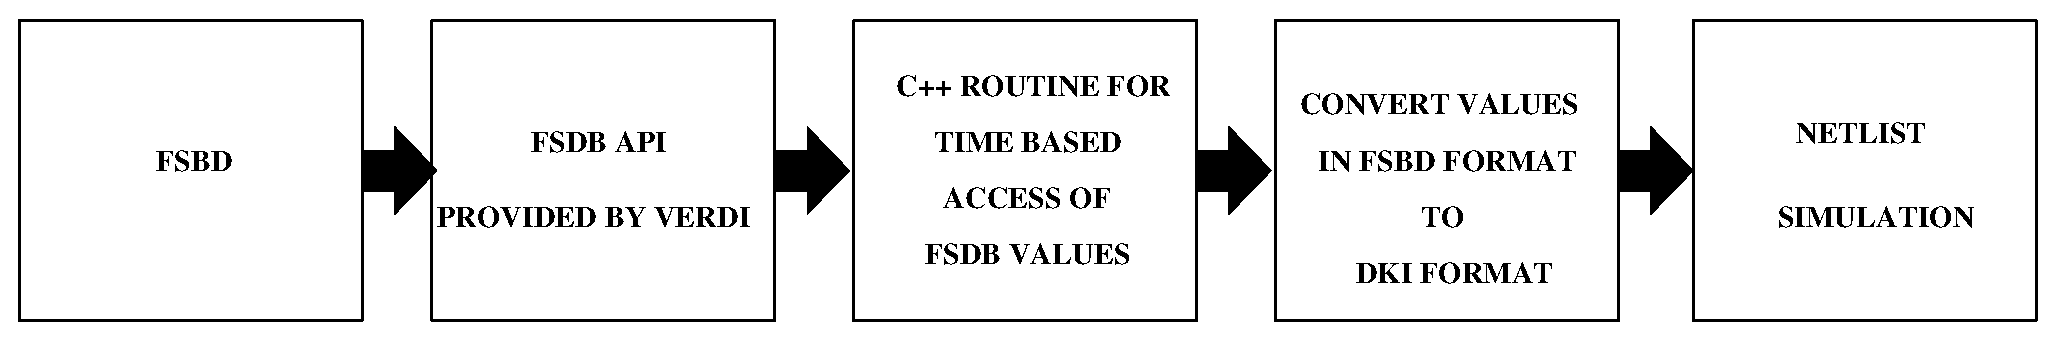
\includegraphics[width=5in, height=3in]{./figures/fsdb.ps}
%=======
%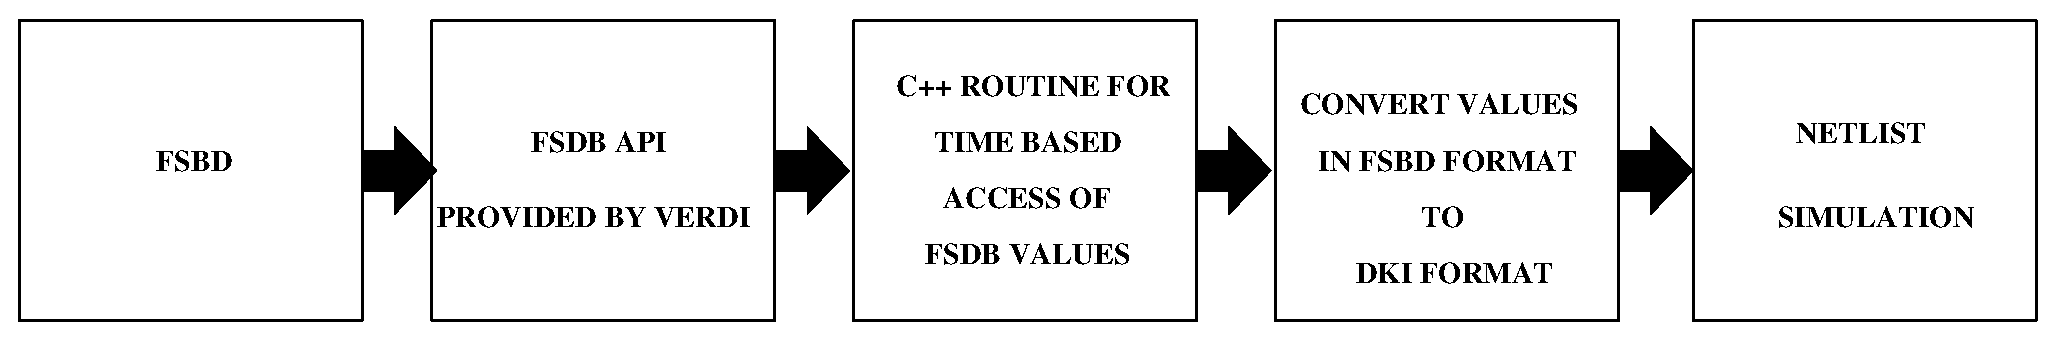
\includegraphics[width=5in, height=1.3in]{./figures/fsdb.ps}
%>>>>>>> 67c22b93efe2b05d3738c447bedb04180afbaae5
\caption{Accessing FSDB Signals}
\label{fig:fsdb.eps}
\end{figure}

~\figurename{~\ref{fig:fsdb.ps}} shows how test vectors are obtained from .fsdb file and attached onto the netlist simulation flow. The various stages involved are explained below.

\paragraph{Extracting data from FSDB:}In FSDB signals are stored in binary format and can be accessed only by specific tools or using some appropriate APIs.  In this project we are using FSDB APIs provided by Verdi. These API's allow us to access each signal separately. 


\begin{figure}[H]
\centering
\includegraphics[width=4.5in, height=3.5in]{./figures/verdi.ps}
\caption{API For Accessing FSDB Signals}
\label{fig:verdi.eps}
\end{figure}






Once the list of RTL signals that need to be extracted is decided, make FSDB signals object handles corresponding to each signal. FSDB signal objects are also defined by the API and allow signals in FSDB file to be attached to these objects. Special "{\emph Attach()}" routines are provided for signal attach with objects.

However just attaching to the signal is not enough. A larger C++ infrastructure is required for accessing signals for gatesim because of the following reasons:
1.	Values contained in FSDB needs to be accessed in time-based fashion.
2.	Typical netlist contained hundreds of stimulus points with many wider bus-signals.
The C++ infrastructure will open the FSDB file and initiate a playback through the file. Whenever a signal that is attached using APIs changes, the C++ will identify this and will ensure the changed value is made available to the netlist simulation.  Figure x shows the complete flow of the C++ routine developed for FSDB signal access, conversion and application onto Verilog component.


\begin{figure}[H]
\centering
\includegraphics[width=6in]{./figures/cpp.ps}
\caption{C++ Routine for FSDB Signal Extraction}
\label{fig:cpp.eps}
\end{figure}




A set of RTL signal accessed at time based manner and applied onto netlist is effectively doing the job of test vectors as vectors are nothing but signal values at different instants of time.
Once signals are accessed from FSDB file by API's and C++ routine developed next step is applying it onto netlist. However Verilog based netlist cannot directly interact with extracted FSDB format objects. For this a conversion stage is required.  




\paragraph{Convert FSDB format to DKI format}: The FSDB format signals are converted to a standard format that can work with Verilog. There are many interfaces that allow Verilog-C interaction such as PLI, VPI (or PLI 2.0) or DKI. 
In this work we are using DKI which is an API that is supported only by VCS. This has the advantage of less simulation overhead and smaller memory footprint compared to VPI interface.
For converting FSDB signal format to DKI format, we are assigning signal values of the FSDB signal object to a corresponding DKI signal object. Similar to the creation of FSDB signal object list, create a DKI object list corresponding to the RTL signals. 

Whenever the C++ moves in time and identify a change in signal value in FSDB signal, an assign statement will assign the new FSDB signal value to DKI signal object.  These DKI signals can drive Verilog signals by using "{\emph Attach}" routine provided by API, that ties together DKI object with RTL signal. 

\subsection{NETLIST SIMULATION FLOW}
In the previous section we have discussed extracting FSDB, accessing it in a time based manner and converting it to a format that can interact with Verilog. Next step is using these signals for netlist simulation.


\begin{figure}[H]
\centering
\includegraphics[width=5in, height=3.5in]{./figures/netlist_sim.ps}
\caption{Netlist Simulation}
\label{fig:netlist_sim.eps}
\end{figure}

~\figurename{~\ref{fig:netlis_sim.eps}} show how test vectors are applied onto the netlist and how final comparison is done.

The test vectors obtained from the FSDB are applied to a dummy RTL module. Dummy RTL module has no logic other than the RTL signal list that are required for netlist simulation, that is the driving Input signals and the output signal for RTL-Netlist output comparison.. The DKI attach will link these empty RTL signals with DKI signal objects, and any change in DKI object is reflected as change in value of the attached dummy RTL signal.




%Features of Improved gatesim methodology are:
%\begin{enumerate}
%	\item Obtain test vectors from FSDB; access it in time-based fashion.
%	\item Drive stimulus onto a dummy RTL. This dummy RTL does not have any logic other than Input/output. All the input and output ports of the module netlist are included in this dummy RTL module. 
%	\item Dummy RTL drives netlist stimulus and other stimulus points inside design (like fuses, un init flops).
%	\item Apply appropriate force signals from FSDB directly on to the dummy RTL. The dummy RTL signal forces the netlist signals.
%	\item Accomplish verification goals by cycle-comparing netlist behavior to that of its counterpart RTL (as available in the FSDB).
%\end{enumerate}
%It should be noted that the improved methodology is still dependent on vectors from RTL simulations and is not independent by itself. But gains obtained in turn-around times were of great benefit.
%


 


%%%%%%%%%%%%%%%%%%%%%%%%%%%%%%%%%%%%%% RESULTS %%%%%%%%%%%%%%%%%%%%%%%%%%%%%%%%%%%%%%%%%%%%%%%
\newpage
\chapter{RESULTS}
\label{chap:results.tex}
A new gate simulation flow based on separate simulation of RTL and netlist was developed. Performance analysis was done with respect to co-sim methodology. A set of standard test cases were considered for the purpose. An exclusive machine was used for benchmarking and hence tests were run in sequence one after the other in both the methodologies. The machine features were:
\begin{itemize}
\item Linux 2.6.18-308.1.1.el5
\item Authentic AMD family F model 1 stepping 2
\item AMD FX(tm)-8150 Eight-Core Processor
\item MemTotal:     32925800 kB
\end{itemize}  

~\tablename{~\ref{tab:Simulation Performance}} compares simulation performances whereous ~\tablename{~\ref{tab:Memory Requirement}} compares simulation memory requirement.
%%%%%%%%%%%%%%%%%%%%%%%%%%%%%%%%%%%%%%%%%%%%%%%%%%%%%%%%%%%%%%%%%%%%%%%%%%%%%%%%%


%%%%%%%%%%%%%%%%%%%%%%%%%%%%%%%%%%%%%%%%%%%%%%%%%%%%%%%%%%%%%%%%%%%%%%%%%%%%%%%%%
\newpage
\section{SIMULATION PERFORMANCE ANALYSIS}
\begin{table}[h!]
\begin{center}
\caption{Simulation Performance Comparison}
\label{tab:Simulation Performance}
\vspace{0.2cm}
\begin{tabular}{|l|r|r|r|}
\hline
\multirow{3}{*}{\bf Stimulus} & &	&\\ & {\bf Co-sim Simulation} 	& {\bf Dual-sim Simulation} & {\bf Improvement } 	\\ & {\bf Time (in sec)}  &  {\bf Time (in sec)} &  {\bf(X times) }\\



%\multirow{2}{*}{\bf Stimulus}	&\multirow{2}{*}{\bf Co-sim Simulation Time (in sec)}	&\multirow{2}{*}{\bf Dual-sim Simulation Time (in sec)}	&\multirow{2}{*}{\bf Improvement (X times)} 		\\
						&				&				&				\\
\hline
Pattern 1 			&821245				&79965				&10.27 				\\
Pattern 2  				&883227				&85731				&10.3 				\\

Pattern 3  		&854760				&83083				&10.28				\\

Pattern 4  			&456881				&46071 				&9.91				\\

Pattern 5  				&709871				&69605				&10.19				\\
\hline


\end{tabular}
\end{center}

\end{table}



\section{MEMORY REQUIREMENT}
\begin{table}[h!]
\begin{center}
\caption{Simulation Memory Requirement}
\label{tab:Memory Requirement}
\vspace{0.2cm}
\begin{tabular}{|l|r|r|r|}
\hline
\multirow{3}{*}{\bf Stimulus} & &	&\\ & {\bf Co-sim Simulation} 	& {\bf Dual-sim Simulation} & {\bf Improvement } 	\\ & \bf{Mem Req (in Mb)}  &  {\bf{Mem Req (in Mb)}} &  {\bf(X times) }\\



%\multirow{2}{*}{\bf Stimulus}	&\multirow{2}{*}{\bf Co-sim Simulation Time (in sec)}	&\multirow{2}{*}{\bf Dual-sim Simulation Time (in sec)}	&\multirow{2}{*}{\bf Improvement (X times)} 		\\
						&				&				&				\\
\hline
Pattern 1 			&1103.9				&98.8				&11.17 				\\

Pattern 2  				&1103.9				&98.8				&11.17				\\

Pattern 3  		&1105.1				&98.8				&11.18				\\

Pattern 4  			&1103.3			&98.8 				&11.17				\\

Pattern 5  				&1103.3				&98.8				&11.17				\\
\hline


\end{tabular}
\end{center}

\end{table}
 

%%%%%%%%%%%%%%%%%%%%%%%%%%%%%%%%%%%%%% CONCLUSION %%%%%%%%%%%%%%%%%%%%%%%%%%%%%%%%%%%%%%%%%%%%%%%
\newpage
\chapter{CONCLUSION}
\label{chap:conclusion}
A new dual-sim or sim after sim flow for gatesim was developed and simulation performances was benchmaked on dedicated machine and compared against current co-simulation method. The simulation performance shows a consistent improvement of around 10 times over the current method. Use of FSDB as the source of test vectors keep the file size small and get rid of bulky time hogging test bench components, and thereby reducing rerun time. This 10 times improvement in simulation performance will help in reducing delay in tape out due to gatesim verification overheads. The method still require a one time RTL simulation run for generating FSDB file. The existing gatesim flow can be maintained as it is and only few changes need to be included in current flow for accommodating the new method. 
\paragraph{Potential for future work:}The performance of dual-sim method can be further increased by improving the VPI/PLI access methods. 


\chapter{REFERENCES}
\bibliographystyle{IEEEtran}
\begin{thebibliography}{10}
\providecommand{\url}[1]{#1}
\csname url@rmstyle\endcsname
\providecommand{\newblock}{\relax}
\providecommand{\bibinfo}[2]{#2}
\providecommand\BIBentrySTDinterwordspacing{\spaceskip=0pt\relax}
\providecommand\BIBentryALTinterwordstretchfactor{4}
\providecommand\BIBentryALTinterwordspacing{\spaceskip=\fontdimen2\font plus
\BIBentryALTinterwordstretchfactor\fontdimen3\font minus
  \fontdimen4\font\relax}
\providecommand\BIBforeignlanguage[2]{{%
\expandafter\ifx\csname l@#1\endcsname\relax
\typeout{** WARNING: IEEEtran.bst: No hyphenation pattern has been}%
\typeout{** loaded for the language `#1'. Using the pattern for}%
\typeout{** the default language instead.}%
\else
\language=\csname l@#1\endcsname
\fi
#2}}
\bibitem{soc}
Mosensoson, Guy,``Practical approaches to SoC verification.''\emph{In Proceedings of DATE User Forum,} pp. 05-08. 2002.

\bibitem{phd:zhang}
Zhang, L. (2005),`` Design Verification for Sequential Systems at Various Abstraction Levels,''\emph{Doctoral dissertation, Virginia Polytechnic Institute and State University,}2005.

\bibitem{ieee:formal:2004}
Tasiran, Serdar, Yuan Yu, and Brannon Batson,``Linking simulation with formal verification at a higher level,''\emph{Design & Test of Computers,} IEEE 21, no. 6, pp. 472-482,2004.

\bibitem{SS:AMD64-V1}
\BIBentryALTinterwordspacing
AMD Corporation (May 2011). ``Volume 1: Application Programming''. \emph{AMD64 Architecture Programmer's Manual}. AMD Corporation. Retrieved 2011-10-29.
\url{http://support.amd.com/us/Processor_TechDocs/24592_APM_v1.pdf}
\BIBentrySTDinterwordspacing
 
\bibitem{SS:AMD64-V2}
\BIBentryALTinterwordspacing
AMD Corporation (May 2011). ``Volume 2: System Programming''. \emph{AMD64 Architecture Programmer's Manual}. AMD Corporation. Retrieved 2011-10-29.
\url{http://support.amd.com/us/Embedded_TechDocs/24593.pdf}
\BIBentrySTDinterwordspacing
 
\bibitem{http:dygraphs}
\BIBentryALTinterwordspacing
Dygraphs. (2013, Jun.) {JavaScript Visualization Ligrary}. [Online]. Available:
  \url{http://dygraphs.com/}
\BIBentrySTDinterwordspacing


\bibitem{ieee:segev:2004}
Segev, Eyal, Sharon Goldshlager, Hillel Miller, Oren Shua, Olga Sher, and Shlomo Greenberg,``Evaluating and comparing simulation verification vs. formal verification approach on block level design,'' \emph{In Electronics, Circuits and Systems, 2004. ICECS 2004. Proceedings of the 2004 11th IEEE International Conference},pp. 515-518, 2004.


\bibitem{ieee:power:2009}
Zhang,~Y., & Zhang,~G. ``Fast gate-level simulation and power analysis for high performance microprocessor,'' in {\emph IEEE Computer Science & Education, 2009. ICCSE'09. 4th International Conference}, pp. 1155-1158, 2009.


\bibitem{ieee:v:2005}
  IEEE,
  \emph{``1364-2005 - IEEE Standard for Verilog Hardware Description
  Language''}.
	IEEE STANDARD,
	2005

\bibitem{ieee:sv:2009}
  IEEE,
	\emph{``1800-2012 - IEEE Standard for SystemVerilog--Unified Hardware Design,
  Specification, and Verification Language''}.
	IEEE STANDARD,
	2009

\bibitem{ieee:boolean}
Randal E. Bryant,
  ``Graph-Based Algorithms for Boolean Function Manipulation,'' \emph{IEEE Transactions on Computers}, vol.C ~35, no.~12, 1986.

\bibitem{lec}
McDonald, William, and Janny Liao,
	``Logic Equivalence Checking Has Arrived For FPGA Developers.`` \emph{Design and Verification Conference (DVCon)}, 2006.

\bibitem{SS:Verdi}
\BIBentryALTinterwordspacing
SpringSoft. (2013, May.) {Verdi Automated Debug System}. [Online]. Available:
  \url{http://www.springsoft.com/products/debug-automation/verdi}
\BIBentrySTDinterwordspacing

	
%\bibitem{compton2002reconfigurable}
%K.~Compton and S.~Hauck, ``Reconfigurable computing: a survey of systems and
%  software,'' \emph{ACM Computing Surveys (csuR)}, vol.~34, no.~2, pp.
%  171--210, 2002.
%
%\bibitem{P1171121623}
%M.~Ramesh~Kini and S.~Sumam~David, ``Asic implementation of address generation
%  unit for digital signal processing kernel-processor,'' \emph{ICGST
%  International Journal on Programmable Devices, Circuits and Systems, PDCS},
%  vol.~11, pp. 1--9, December 2011.
%
%\bibitem{graham1999reconfigurable}
%P.~Graham and B.~Nelson, ``Reconfigurable processors for high-performance,
%  embedded digital signal processing,'' in \emph{Proceedings of 9th
%  international workshop on Field Programmable Logic and Applications}.\hskip
%  1em plus 0.5em minus 0.4em\relax Springer, 1999, pp. 1--10.
%
%\bibitem{ramesh2009comprehensive}
%M.~Ramesh~Kini and S.~Sumam~David, ``Comprehensive address generator for
%  digital signal processing,'' in \emph{Proceedings of International Conference
%  on Industrial and Information Systems (ICIIS 2009),Srilanka}.\hskip 1em plus
%  0.5em minus 0.4em\relax IEEE, 2009, pp. 325--330.
%
%\bibitem{huang2002reconfigurable}
%Z.~Huang and S.~Malik, ``Exploiting operation level parallelism through
%  dynamically reconfigurable datapaths,'' in \emph{Proceedings of the 39th
%  annual Design Automation Conference}.\hskip 1em plus 0.5em minus 0.4em\relax
%  ACM, 2002, pp. 337--342.
%
%\bibitem{SS:AMD64}
%\BIBentryALTinterwordspacing
%AMD64 Architecture Programmer's Manual Volume 1: Application Programming (2005, Nov)
%\url{http://www.serc.iisc.ernet.in/facilities/ComputingFacilities/systems/tyrone/Application\%20Programming.pdf}
%\BIBentrySTDinterwordspacing
\bibitem{SS:Cadence}
\BIBentryALTinterwordspacing
Cadence. (2013, Jan.) {Functional Verification Survey-{\emph Why Gate-Level Simulation is Increasing}}.[Online]. Available:
\url {http://www.cadence.com/Community/blogs}
\BIBentrySTDinterwordspacing

\bibitem{SS:Cadence-2}
\BIBentryALTinterwordspacing
Cadence. (2012, Jan.) {Gate-Level Simulation Methodology-{\emph Improving Gate-Level Simulation Performance}}.[Online]. Available:
\url {http://www.cadence.com/rl/Resources/white_papers/Gate_Level_Simulation_WP.pdf}
\BIBentrySTDinterwordspacing


\bibitem{Verdi:FsdbReader}
\BIBentryALTinterwordspacing
Novas. (2011, Oct.) [Tool Installation Resources]. Available:
  \verb|$VERDI_HOME/share/FsdbReader/doc/FsdbReader.pdf|
\BIBentrySTDinterwordspacing

\bibitem{VCS:vcs.pdf}
\BIBentryALTinterwordspacing
Synopsys. (2013, Dec.) [Tool Installation Resources]. Available:
  \verb|$VCS_HOME/doc/UserGuide/pdf/vcs.pdf|
\BIBentrySTDinterwordspacing

\bibitem{wiki:2013:VPI}
\BIBentryALTinterwordspacing
Wikipedia. (2013, June.) {Verilog Procedural Interface}. [Online]. Available:
  \url{http://en.wikipedia.org/wiki/Verilog_Procedural_Interface}
\BIBentrySTDinterwordspacing

\bibitem{aw:2013:VPI}
\BIBentryALTinterwordspacing
Asic World. (2013, June.) {Verilog Procedural Interface}. [Online]. Available:
  \url{http://www.asic-world.com/verilog/pli6.html}
\BIBentrySTDinterwordspacing

\bibitem{aw:2013:vbooks}
\BIBentryALTinterwordspacing
Asic World. (2013, June.) {Verilog Books}. [Online]. Available:
  \url{http://www.asic-world.com/verilog/books.html}
\BIBentrySTDinterwordspacing

\bibitem{ss:pli:1999}
\BIBentryALTinterwordspacing
Sutherland, Stuart.  {\em The Verilog PLI Handbook: A User's Guide and Comprehensive
  Reference on the Verilog Programming Language Interface}.
\newblock Springer, 1999. Hardcover.
\newblock ISBN: 0-7923-8489-X.
\BIBentrySTDinterwordspacing

\bibitem{sm:pli:1999}
\BIBentryALTinterwordspacing
Mittra, Swapnajit.  {\em Principles of Verilog PLI}.
\newblock Springer, 1999. Hardcover.
\newblock ISBN: 0-7923-8477-6
\BIBentrySTDinterwordspacing

%\bibitem{tms320c55x2001programmer}
%T.~DSP, ``Programmer’s guide,'' \emph{SPRU376, Texas Instruments}, 2001.
%
%\bibitem{EDKconceptsUG683}
%Xilinx, ``Edk concepts, tools, and techniques,'' \emph{UG683 (v12.3), Xilinx},
%  Sept. 2010.
%
%\bibitem{chipscopeguideUG029}
%Xilinx, ``Chipscope pro 12.1 software and cores,'' \emph{UG029 (v12.1),
%  Xilinx}, Apr. 2010.
%
%\bibitem{dorairaj2005planahead}
%N.~Dorairaj, E.~Shiflet, and M.~Goosman, ``Planahead software as a platform for
%  partial reconfiguration,'' \emph{Xcell Journal}, vol.~55, pp. 68--71, 2005.
%
%\bibitem{oslibref}
%Xilinx, ``Xilinx OS and Libraries document collection,'' \emph{UG643, Xilinx},
%  April. 2012.

\end{thebibliography}

%\addcontentsline{toc}{section}{REFERENCES}
\bibliography{reference}

%%%%%%%%%%%%%%%%%%%%%%%%%%%%%%%%%%%%%% BIO DATA %%%%%%%%%%%%%%%%%%%%%%%%%%%%%%%%%%%%%%%%%%%%%%%%%%%%%
\newpage
\pagestyle{plain}

\section*{\centering BIODATA}
\begin{tabular}{lll}
%\begin{center}
Name			&:	&Meera Mohan			\\

Qualification 		&:	&B.Tech (Electronics and Communication)	\\

			&	&Mahatma Gandhi University, Kottayam			\\

Contact Address 	&:	&D/O Mohandas. E. K			\\
		
			&	&Margangattu House		\\
		
			&	&Memana, Oachira		\\

			&	&Kollam, Kerala-690526		\\

Contact Number  	&:	&7411352081				\\

Email id		&:	&miramohan@gmail.com			\\

%List of publications 	&:	&1					\\
%\end{center}
\end{tabular}
%\addcontentsline{toc}{section}{BIODATA}



%\hskip 1em plus
%  0.5em minus 0.4em\relax IEEE, 2009, pp. 325--330.

\end{document}          
